\documentclass[conference]{IEEEtran}
\IEEEoverridecommandlockouts
% The preceding line is only needed to identify funding in the first footnote. If that is unneeded, please comment it out.
%Template version as of 6/27/2024

\usepackage{cite}
\usepackage{amsmath,amssymb,amsfonts}
\usepackage{graphicx}
\usepackage{textcomp}
\usepackage{xcolor}
\usepackage{hyperref}
\renewcommand\UrlFont{\color{blue}\rmfamily}
\usepackage{xspace}
\usepackage[ruled]{algorithm}
\usepackage{booktabs} 
\usepackage{multirow}
\usepackage{array}
\usepackage{diagbox}
\usepackage{makecell}
\usepackage{algorithmic}
\usepackage{threeparttable}
\usepackage{subcaption}

\newtheorem{definition}{\bf Definition}
\newtheorem{lemma}{\bf Lemma}
\newtheorem{theorem}{\bf Theorem}
\newtheorem{proof}{\bf Proof}
%%%%%%%%%%%%%%%%%%%%%%%%%%%%%%%%%%%%%%%%%%%%%%%%%
%comend for REN
\newcommand{\bab}{\textsc{BaB}\xspace}
\newcommand{\abcrown}{$\alpha\beta$-CROWN\xspace}
\newcommand{\ren}{\textsc{REN}\xspace}
\newcommand{\nncs}{\textsc{NNCS}\xspace}
\newcommand{\mle}{\textsc{MLE}\xspace}
\newcommand{\roa}{\textsc{ROA}\xspace}
\newcommand{\ra}{\textsc{RA}\xspace}
%%%%%%%%%%%%%%%%%%%%%%%%%%%%%%%%%%%%%%%%%%%%%%%%%
\newcommand{\myvec}[1]{\boldsymbol{#1}}
\newcommand{\mymatrix}[1]{\boldsymbol{#1}}
\newcommand{\comp}{\mathrel{\circ}}
\newcommand{\relu}{ReLU\xspace}
\newcommand{\combin}[2]{\binom{#1}{#2}}

\newcommand{\red}[1]{\textcolor{red}{#1}}
\newcommand{\todo}[1]{\red{TODO: #1}}
\newcommand{\jx}[1]{\red{Jiaxiang: #1}}
\newcommand{\notsure}[1]{\textcolor{red}{#1}}

% Special fonts
\newcommand{\calA}{\mathcal{A}}
\newcommand{\calB}{\mathcal{B}}
\newcommand{\calC}{\mathcal{C}}
\newcommand{\calD}{\mathcal{D}}
\newcommand{\calG}{\mathcal{G}}
\newcommand{\calS}{\mathcal{S}}
\newcommand{\calP}{\mathcal{P}}
\newcommand{\calQ}{\mathcal{Q}}
\newcommand{\calK}{\mathcal{K}}
\newcommand{\calL}{\mathcal{L}}
\newcommand{\calU}{\mathcal{U}}
\newcommand{\calN}{\mathcal{N}}
\newcommand{\calX}{\mathcal{X}}
\newcommand{\calY}{\mathcal{Y}}
\newcommand{\bbB}{\mathbb{B}}
\newcommand{\bbD}{\mathbb{D}}
\newcommand{\bbR}{\mathbb{R}}
\newcommand{\bbN}{\mathbb{N}}

\def\BibTeX{{\rm B\kern-.05em{\sc i\kern-.025em b}\kern-.08em
    T\kern-.1667em\lower.7ex\hbox{E}\kern-.125emX}}

\begin{document}

% \title{Robustness Evaluation for NNCS 
% with different distribution functions}

\title{Robustness Evaluation for NNCS 
with different distribution functions
\thanks{This work is partially supported by 
  \todo{Question for JiangTao Li}.}}

\author{\IEEEauthorblockN{1\textsuperscript{st} Given Name Surname}
\IEEEauthorblockA{\textit{dept. name of organization (of Aff.)} \\
\textit{name of organization (of Aff.)}\\
City, Country \\
email address or ORCID}
\and
\IEEEauthorblockN{2\textsuperscript{nd} Given Name Surname}
\IEEEauthorblockA{\textit{dept. name of organization (of Aff.)} \\
\textit{name of organization (of Aff.)}\\
City, Country \\
email address or ORCID}
\and
\IEEEauthorblockN{3\textsuperscript{rd} Given Name Surname}
\IEEEauthorblockA{\textit{dept. name of organization (of Aff.)} \\
\textit{name of organization (of Aff.)}\\
City, Country \\
email address or ORCID}
}

\maketitle

\begin{abstract}
    The robustness of Neural Networks (NNs) 
    is important in security. 
    A considerable works employ the lower bound on 
    minimum distortion on the 
    robustness of classification NNs. 
    Compared to classification NNs, 
    Neural Network Controlled Systems (\nncs) 
    are more complex and 
    are more pertinent to security. 
    % However, the construction 
    % of \nncs challenges the 
    % detection and application of its 
    % precise minimum distortion. 
    However, a gap exists in 
    establishing a framework for 
    the lower bound on 
    minimum distortion in \nncs. 
    To fill this gap and offer support for 
    future works, we provide one of 
    the properties of \nncs, 
    the lower bound on its minimum distortion, 
    for all states of interest with soundness. 
    This paper demonstrates that 
    \nncs adheres to Lipschitz continuity under 
    general conditions. Subsequently, 
    we utilize this continuity to delineate a 
    lower bound for the minimum distortion 
    of \nncs.
    More importantly, this paper proves that 
    the distribution of the Lipschitz constant 
    varies with the running time 
    of \nncs and uses probability approaches to compute 
    the lower bound. 
    This framework is 
    termed the \textbf{R}obustness
    \textbf{E}valuation for 
    \textbf{N}\textsc{NCS}\xspace 
    framework (\ren). 
    Experiments validate that our framework 
    is a promising work which can 
    offer a lower bound on minimum distortion 
    within both theoretical and applied domains.
    % Experimental results validate the 
    % properties proved in our work. 
    % Furthermore, the \ren framework 
    % improves the average 
    % efficiency of SOTA verification 
    % in dichotomy for detecting 
    % the minimum distortion of
    % \nncs by \todo{Number}, 
    % indicating that the \ren 
    % is a promising framework with 
    % the capability to 
    % facilitate the detection of the 
    % precise minimum distortion in \nncs.
    % Source code at \url{https://github.com/XuezhouTang/REN}. 
\end{abstract}

\begin{IEEEkeywords}
Neural Network Controlled Systems, Lipschitz continuity, 
Probability distribution function
\end{IEEEkeywords}

\section{Introduction}
Neural networks (NNs) are 
extensively applied in the 
Internet of Things (IoT) 
vehicles~\cite{pacheco2016iot,naveed2024towards}, 
Large Language Models (LLMs) 
\cite{morales2024dsl,chen2023automated}, 
% as well as 
% code completion~\cite{ciniselli2024deep} and 
software maintaining  
\cite{ayoughi2024enhancing,weber2024model}, and so on. 
These applications are intrinsically linked to 
the security of individuals.
The assertion that the inherent uncertainty of 
NNs renders them susceptible to perturbations, 
thereby posing security risks, 
has been demonstrated in several 
studies~\cite{kaufmann2020deep,madry2017towards}.
For instance, manipulated traffic signs could mislead specific autonomous driving systems, 
resulting in erroneous 
predictions~\cite{morgulis2019fooling}. 
The minimum perturbation that 
induces an unsafe situation 
is termed minimum 
distortion~\cite{weng2018evaluating}, which 
reflects the robustness of NN. 
Additionally, the lower bound on 
minimum distortion of NNs 
serves as a role for training more robust 
classification NNs~\cite{silva2020opportunities,amini2021robust,zhou2022adversarial,wang2024survey}, 
improving attack or defence methods~\cite{bai2021recent,zhao2024attack}, 
evaluations~\cite{weng2018evaluating}, and so on. 

% The complex non-linear 
% input-output relationships in NNs challenge the 
% verification process~\cite{katz2017reluplex}. 
% Despite the existence of mature methods for analyzing 
% the robustness of NNs and identifying 
% the minimum distortion~\cite{xu2020fast,bunel2020branch,tang2023boosting,singhbeyond}, 
% these methods typically demand considerable 
% resources~\cite{ugare2023incremental,tang2024improved}. 
% Considering the costs and hardware constraints, 
% their deployment in practical development remains 
% challenging~\cite{DBLP:conf/cav/HuangKWW17,DBLP:journals/csr/HuangKRSSTWY20,yahmed2023deploying}. 

In the fields of control theory, 
such as IoT vehicles~\cite{pacheco2016iot,sathiyanarayanan2018smart} 
and drones~\cite{hassanalian2017classifications,saunders2024autonomous}, 
there is a growing trend to substitute traditional 
controllers with 
NNs~\cite{nubert2020safe,abu2022deep,kohler2020computationally}, 
resulting in systems termed Neural 
Network Controlled Systems (\nncs).
In practical applications, \nncs demonstrates 
enhanced efficiency, improved security performance, 
and greater adaptability to environmental 
changes~\cite{liu2023modeling,kohler2020computationally}.
% As \nncs are based on NNs, 
% they exhibit a similar sensitivity to 
% perturbations~\cite{tian2023taming}. 
% Therefore, 
\nncs 
are closely tied to the security of 
human life and property, 
necessitate guarantees on robustness.

Recently, the verification of 
\nncs has attracted 
significant interest, prompting 
several verification initiatives 
\cite{ivanov2021verisig,huang2022polar,sha2021synthesizing}. 
% Studies by 
% aim to compute the bounds of the reachability 
% through linearizing the non-linear relations in \nncs. 
% By comparing the bounds with the predefined target region, 
% the robustness of the \nncs can be estimated. 
Verification efforts by 
\cite{xue2020inner,xue2021reach,zhang2023reachability} 
inner-approximate the reach-avoid set (\ra) to ensure the 
security of \nncs. The calculation of precise 
\ra is NP-hard~\cite{xue2020inner}. 
\ra is approximated through the 
construction of barrier functions, which 
delineate safe conditions of the \nncs. 
% The barrier function is obtained by predefined 
% region of interest, target region, and 
% safe region~\cite{vzikelic2023learning,zhi2024unifying}. 

Meanwhile, several works 
further the barrier function of \ra 
in control theory. 
Their barrier function 
inner-approximates the region-of-attraction (\roa) 
\cite{dai2021lyapunov,wu2023neural,yanglyapunov}. 
\roa is widely used in control fields such as 
stability analysis~\cite{chakraborty2011nonlinear,chen2014stability}, 
controller design~\cite{korda2014controller,mauroy2016global}, 
robustness verification~\cite{wu2023neural,yanglyapunov} and so on.
The calculation of the 
precise \roa 
is also NP-hard~\cite{dai2021lyapunov}. 
\roa is proposed according to the 
Lyapunov stability~\cite{lyapunov1992general} in control theory 
offering a robust framework to verify the closed-loop 
stability of dynamical systems~\cite{yanglyapunov}. 
% In these studies, the required predefined input 
% is the region of interest\cite{dai2021lyapunov}. 
% the target and safe domain required in \ra 
% methods can be implied by the Lyapunov conditions. 

The lower bound on minimum distortion 
provided by barrier functions is 
limited within the domain of states 
under consideration and 
overestimated due to inner-approximation, 
as detailed in Exp \ref{exam:efficiency}. 
Consequently, a gap persists 
in determining the lower bound for minimum 
distortion for all states of interest within \nncs.

% If the initial 
% state $\myvec{x}$ lies outside 
% the trained inner-approximation of \ra (or \roa), 
% the lower bound on the minimum 
% distortion for $\myvec{x}$ cannot 
% be determined. Consequently, 
% a framework for estimating the lower bound 
% of minimum distortion for all 
% $\myvec{x}$ of interested in \nncs is essential.

% Nevertheless, because \nncs is a kind of time-variant systems, 
% which are inherently more complex than 
% neural networks. Consequently, the verification 
% of their robustness or minimum distortion is prone to constraints 
% imposed by computational expense, hardware limitations, 
% or sampling constraints~\cite{ivanov2021verisig,huang2022polar}.

Due to the fact that 
the calcualtion of the \ra or \roa 
is NP-hard, it is challenging 
to obtain the precise minimum distortion 
of \nncs. 
% current studies 
% provide only inner-approximations of 
% the \ra or \roa, it is challenging to 
% utilize their barrier functions to 
% accurately identify the minimum 
% distortion in \nncs. 
% This challenge causes a less 
% comprehensive application of robustness 
% in \nncs compared to its application 
% in classification NNs. 
Presently, attack methods 
\cite{weng2018evaluating, zhao2024attack} can 
estimate the upper bound on 
the minimum distortion for \nncs~\cite{weng2018evaluating}. 
However, a gap exists in 
establishing the sound lower bound on the 
minimum distortion for \nncs which is more 
applicable than upper bound from attacks~\cite{wang2024survey}. 
To fill this gap, 
our method focuses on providing 
% the region-of-attraction (\roa) within 
the lower bound on minimum distortion in \nncs 
within either \ra or \roa's barrier functions 
for all state of interest. 
% \roa is proposed according to the 
% Lyapunov stability~\cite{lyapunov1992general} in control theory 
% offering a robust framework to verify the closed-loop 
% stability of dynamical systems~\cite{yanglyapunov}. 
The distribution that governs this lower bound 
is then proven to mitigate the risks 
due to sampling uncertainty. 
Experiments validate that our framework 
is a promising work which can 
offer a lower bound on minimum distortion 
within both theoretical and applied domains.

% It should be acknowledged that discrete-time \nncs 
% are generally applied in tasks such as 
% robot control and Programmable Logic 
% Controller (PLC) operations~\cite{vidal1988implementing,nubert2020safe}. 
% Consequently, SOTA studies on \nncs verification 
% utilizing the region-of-attraction (\roa) is 
% predicated on discrete-time \nncs. 
% This paper also analysis \nncs in a 
% discrete-time framework, as 
% it draws upon the conclusions 
% provided by current verification tools~\cite{yanglyapunov} 
% within \roa. 
% To the best of our knowledge, this is the 
% first approach to employ the 
% Lipschitz constant to derive a 
% lower bound on minimum distortion for \nncs. 

% This framework not only enhances the efficiency of minimum 
% distortion search through verification 
% but also identifies a more precise minimum 
% distortion than attack methods, 
% while incurring a comparable computational cost.
% This approach not only improves the efficiency 
% of verification but also optimizes 
% the performance of verification and attack.

The key contributions of this work include:
\begin{itemize}
    \item 
    We establish 
    that \nncs exhibits Lipschitz continuity under 
    general conditions in two different scenarios
    (state/output feedback control) in Theorem~\ref{theorem:nncs Lipschitz continuity}. 
    Subsequently, we derive a lower bound for 
    the minimum distortion of \nncs in Theorem~\ref{theorem:Robustness evaluation for NNCS}. 
    % based on the definition of the \roa and 
    % the Lipschitz continuity of \nncs. 
  
    \item 
    We demonstrate that the Lipschitz constant 
    invoked in the lower bound for 
    minimum distortion of \nncs obeys 
    One-point distribution or a non-degenerate cumulative distribution 
    according to the duration(or time steps) of the 
    \nncs in Theorem~\ref{theorem:different distributions}. 
    Then we use probability approaches 
    to compute this lower bound which 
    is the robustness evaluation 
    in our \ren framework. 
  
    \item 
    We realize our proposed framework \ren 
    and evaluate it on several 
    standard tasks for \nncs. 
    The experiments validate the distribution 
    properties established by our study and 
    % confirm the observations on the lower bound 
    % of minimum distortion generated by barrier 
    % functions, thereby distinguishing 
    distinguish the \ren framework from 
    the barrier functions. 
    Comparative results reveal that the 
    \ren framework provides a practical and sound 
    lower bound. 
    
  \end{itemize}

\paragraph{Organaization.}
Sec~\ref{sec:pre} provides the preliminaries. 
% on neural network controlled systems (\nncs)  
% , definitions of reach-avoid set(\ra) and 
% region of attraction (\roa). 
Our methodology and proofs are detailed in Sec~\ref{sec:method} 
and Sec~\ref{sec:algorithm}. 
Experiments are estimated in Sec~\ref{sec:exp}. 
Sec~\ref{sec:conclusion} concludes this paper. 

\section{Preliminaries}\label{sec:pre}
This section provides the notions about \nncs, 
the definitions of \ra and \roa. 

\subsection{Neural Network Controlled Systems (\nncs)}
We discuss a nonlinear discrete-time system 
generally applied in tasks such as 
robot control and Programmable Logic 
Controller (PLC) operations 
\cite{vidal1988implementing,nubert2020safe} 
with the following plant:
\begin{subequations}
  \begin{align}
    \myvec{x}_{t+1} = f(\myvec{x}_{t},\myvec{u}_{t}), \label{eq:plant1} \\
    \myvec{y}_{t} = \myvec{h}(x_{t}). \label{eq:plant2}
  \end{align}
\end{subequations}
where $\myvec{x}_{t} \in \bbR^{n_{\myvec{x}}}$ denotes the state of the \nncs at time step $t, t\in \bbN$, 
$\myvec{u}_{t} \in \bbR^{n_{\myvec{u}}}$ represents 
the control input or action produced by the controller, 
which is a component of the \nncs, 
and the $\myvec{y}_{t} \in \bbR^{n_{\myvec{y}}}$ constitutes the output of the system. 
In the context of discrete-time \nncs research, 
the continuity of systems in reality needs to be considered. 
As a result, current state-of-the-art studies uniformly assume that the dynamic functions 
$f(\myvec{x}_{t},\myvec{u}_{t})$ and $h(\myvec{x}_{t})$
are continuous with respect to both 
$\myvec{x}_{t}$ and $\myvec{u}_{t}$~\cite{luenberger1971introduction,xue2020inner,meyn2022control}. 
This work adheres to this assumption. 
We discuss two kinds of 
discrete-time \nncs :

\subsubsection{State feedback control}
In this scenario, the system only has a plant and a 
controller $\pi$ parameterized by neural networks 
$\phi_{\pi}:\bbR^{n_{\myvec{x}}} \to \bbR^{n_{\myvec{u}}}$. 
This configuration is depicted in the left of 
Fig~\ref{fig:two_feedback_secnarios}. 
The state feedback controller is defined as follows:
\begin{equation}\label{eq:state_feedback_control}
\myvec{u}_{t} = \pi(\myvec{x}_{t}) = 
\phi_{\pi}(\myvec{x}_{t}) - \phi_{\pi}(\myvec{x}^{\star}) + 
\myvec{u}^{\star}.
\end{equation}
Here, $\myvec{x}^{\star}$ denotes the equilibrium state, 
generally a zero-filled vector, 
$\myvec{0}_{n_{\myvec{x}}} \in \bbR^{n_{\myvec{x}}}$. 
Additionally, $\myvec{u}^{\star} \in \bbR^{n_{\myvec{u}}}$ represents the 
action at equilibrium. 
\begin{figure}[htbp]
    \centerline{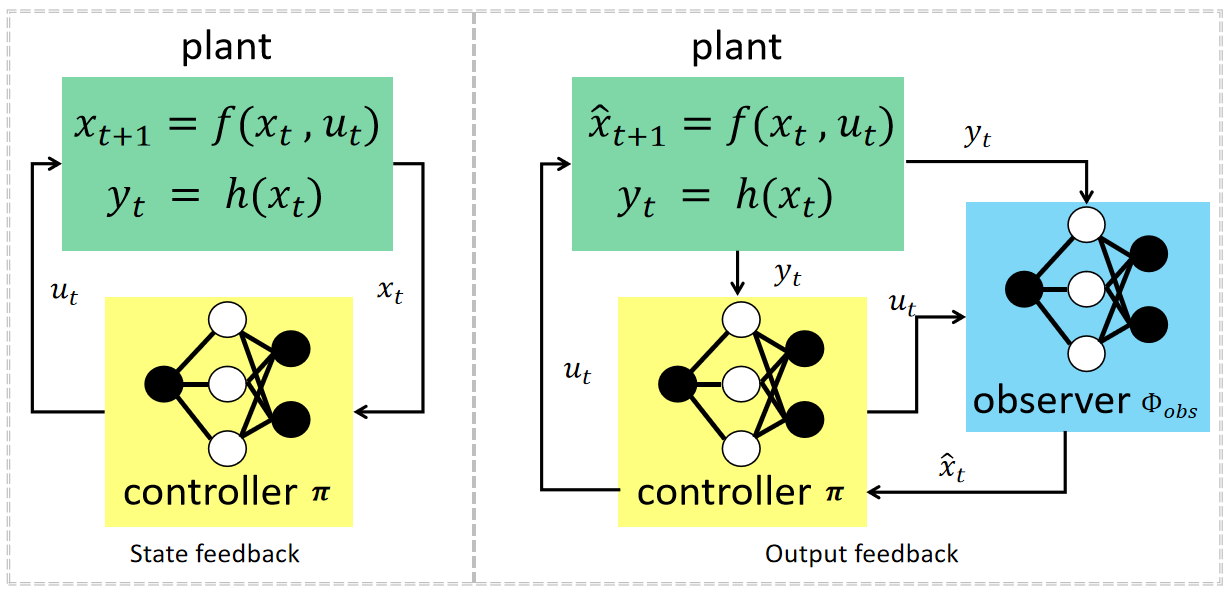
\includegraphics[width=0.9\columnwidth]{figures/feedback.png}}
    \caption{In state feedback secnario, the \nncs has a plant and a controller 
    implemented by a neural network $\pi$. In output feedback secnario, the \nncs has a plant, a controller neural network $\pi$, 
    and an observer neural network $\phi_{obs}$.}
    \label{fig:two_feedback_secnarios}
\end{figure}

\subsubsection{Output feedback control}
In output feedback secnario, an additional model named 
observer is considered in \nncs, 
shown on the right of Fig~\ref{fig:two_feedback_secnarios}. 
The observer is instrumental in mitigating errors 
both within and beyond the model~\cite{luenberger1971introduction,crary1990techniques,chen2015disturbance}. 
It utilizes system input and output data  
to estimate unmeasurable internal states:
% \begin{equation}\label{eq:output_feedback_state}
% \hat{\myvec{x}}_{t+1} = 
% f(\hat{\myvec{x}}_{t}, \myvec{u}_{t}) + 
% \phi_{obs}(\hat{\myvec{x}}_{t}, \myvec{y} - \myvec{h}(\hat{\myvec{x}}_{t})) 
% - \phi_{obs}(\hat{\myvec{x}}_{t}, \myvec{0}_{n_{\myvec{y}}}).
% \end{equation}

% \begin{equation}\label{eq:output_feedback_control}
%   \myvec{u}_{t} = \pi(\hat{\myvec{x}}_{t}, \myvec{y}_{t}) = 
% \phi_{\pi}(\hat{\myvec{x}}_{t},\myvec{y}_{t}) - 
% \phi_{\pi}(\myvec{x}^{\star},\myvec{h}(\myvec{x}^{\star})) + 
% \myvec{u}^{\star}.
% \end{equation}
\begin{subequations}
  \begin{align}
    &\hat{\myvec{x}}_{t+1} = 
    f(\hat{\myvec{x}}_{t}, \myvec{u}_{t}) + 
    \phi_{obs}(\hat{\myvec{x}}_{t}, \myvec{y} - \myvec{h}(\hat{\myvec{x}}_{t})) 
    - \phi_{obs}(\hat{\myvec{x}}_{t}, \myvec{0}_{n_{\myvec{y}}}), \label{eq:output_feedback_state} \\
    &\myvec{u}_{t} = \pi(\hat{\myvec{x}}_{t}, \myvec{y}_{t}) = 
    \phi_{\pi}(\hat{\myvec{x}}_{t},\myvec{y}_{t}) - 
    \phi_{\pi}(\myvec{x}^{\star},\myvec{h}(\myvec{x}^{\star})) + 
    \myvec{u}^{\star}. \label{eq:output_feedback_control}
  \end{align}
\end{subequations}
where $\hat{\myvec{x}}\in \bbR^{n_{\myvec{x}}}$ 
represents the estimated state derived from the observer. 
According to the Luenberger 
observer~\cite{luenberger1971introduction} 
invoked in Yang et.al~\cite{yanglyapunov}, 
$\hat{\myvec{x}}_{0} = \mymatrix{H}\myvec{x}_{0}$, 
$\mymatrix{H}\in \bbR^{n_{\myvec{x}}} \times \bbR^{n_{\myvec{x}}}$ 
is a set matrix. 
The function $\phi_{obs}:\bbR^{n_{\myvec{x}}} \times 
\bbR^{n_{\myvec{y}}} 
\to \bbR^{n_{\myvec{x}}}$ constitutes a neural network 
that supplants the conventional observer process, 
as detailed in ~\cite{luenberger1971introduction}. 
% It is evident from Eqs. (\ref{eq:output_feedback_state}) 
% and (\ref{eq:output_feedback_control}) that if 
% the condition $\hat{\myvec{x}}_{t} = \myvec{x}_{t}$ is 
% satisfied, then $\hat{\myvec{x}}_{t+1} = \myvec{x}_{t+1}$ 
% will hold true. 

\subsubsection{Union formulation}
In the following, 
we introduce the union formulation~\cite{yanglyapunov} 
for the state and output feedback scenarios, 
which is based on an internal state 
$\myvec{\xi}_{t} \in \bbR^{n_{\myvec{\xi}}}$ 
and the dynamic function 
$\myvec{\xi}_{t+1}=f_{d}(\myvec{\xi}_{t})=
f_{d}^{(t+1)}(\myvec{\xi}_{0})$, 
to facilitate the analysis. 

For state feedback secnario, 
there is simply $\myvec{\xi}_{t} = \myvec{x}_{t}$ and:
\begin{equation}\label{eq:state_feedback_dynamic}
  f_{d}(\myvec{\xi}_{t}) = 
  f(\myvec{\xi}_{t}, \pi(\myvec{\phi}_{t})).
\end{equation}

For output feedback secnario, 
the internal state $\myvec{\xi}_{t} = [\myvec{x}_{t},\myvec{e}_{t}]^{T}$, 
where $\myvec{e}_{t} = \hat{\myvec{x}}_{t} - \myvec{x}_{t}$ is the 
prediction error. 
The $\myvec{\xi}_{t}$ is a verctor function of state $\myvec{x}_{t}$. 
The dynamic function is defined as:
\begin{equation}\label{eq:output_feedback_dynamic}
  f_{d}(\myvec{\xi}_{t}) = \begin{bmatrix}
    f(\myvec{x}_{t}, \pi(\myvec{x}_{t}, \myvec{h}(\myvec{x}_{t}))), \\ 
    f(\myvec{x}_{t}, \pi(\hat{\myvec{x}_{t}}, \myvec{h}(\myvec{x}_{t}))) + 
    \myvec{g}(\myvec{x}_{t}, \hat{\myvec{x}}_{t}) 
    - \myvec{x}_{t}
    \end{bmatrix}.
\end{equation}
where $\myvec{g}(\myvec{x}_{t}, \hat{\myvec{x}}_{t}) = 
\phi_{obs}(\hat{\myvec{x}}_{t}, \myvec{h}(\myvec{x}_{t}) - 
\myvec{h}(\hat{\myvec{x}}_{t})) - \phi_{obs}(\hat{\myvec{x}}_{t}, 
\myvec{0}_{n_{\myvec{y}}})$. 
%%%%%%%%%%%%%%%%%%%%%%%%%%%%%%%%%%%%%%%%%%%%%%%%%%

\subsection{Reach-Avoid set}

Under the discrete-time systems with 
dynamics~(\ref{eq:state_feedback_dynamic}) or 
(\ref{eq:output_feedback_dynamic}), 
the Reach-Avoid set 
(\ra)~\cite{xue2020inner,xue2021reach} 
enables any state starting 
from \ra to reach a target set TR in finite 
time while staying within a compact 
set $\calB \in \myvec{X}$ until 
the target is hitten, where $\myvec{X} = 
\{\myvec{x}\in \mathbb{R}^{\myvec{x}}
|h_b(\myvec{x}<1)\}$ 
is the region of all states in the secnario. 

\begin{definition}($\textbf{Reach-Avoid Set}\ (\ra)$~\cite{xue2020inner}). 
  The reach-avoid set \ra is 
  the set of all states which 
  achieve the target set TR at 
  finite time $t \in \mathbb{N}$ while 
  maintaining in the set $\calB$ over the 
  time horizon $[0,t] \cap \mathbb{N}$, i.e., 
  \begin{equation}
    RA=\{\myvec{x}_{0} \in \calB | 
    \exists t \in \mathbb{N}, \myvec{x}_{t}\in 
    TR \wedge \bigwedge^{t}_{j=1}\myvec{x}_{j} 
    \in \calB \}\label{eq:RA 1}
  \end{equation}
\end{definition}
where TR and $\calB$ are 
defined by polynomial inequations
\begin{subequations}
  \begin{align}
    &TR = \{ \myvec{x} \in \mathbb{R}^{\myvec{x}} | g(\myvec{x}) < 1 \} \label{eq:RA 2}\\
    &\calB = \{ \myvec{x} \in \mathbb{R}^{\myvec{x}} | h_{0}(\myvec{x}) \leq 0 \}\label{eq:RA 3}
  \end{align}
\end{subequations}
The $g(\myvec{x}),\ h_{0}(\myvec{x}) \in \mathbb{R}[\myvec{x}]$ 
and $TR \subset \calB$, 
where $\mathbb{R}[\myvec{x}]$ means the 
polynomial ring with respect to $\myvec{x}$ which 
is smooth to $\myvec{x}$. 
The \ra set is inner-approximated in Xue et al. as 
$\calS=\{\myvec{x}\in \calB|V(\myvec{x})<1\}$, 
$\calS \subset \ra$ where
\begin{equation}\label{eq:RA 4}
  V(\myvec{x}) := lim_{t \rightarrow \infty}inf\ \frac{\sum_{i=0}^{t-1}g(\myvec{x}_{i})}{t}
\end{equation}
The barrier function $1-V(\myvec{x})$ in 
Xue et al~\cite{xue2020inner} 
inner-approximates the \ra 
through following optimization: 
\begin{subequations}
  \begin{align}
    max\ &\myvec{c}\cdot \myvec{w} \label{eq:lapunov optimization} \\
    s.t.&V(\myvec{x}) - V(f(\myvec{x})) + s_0(\myvec{x})h_{0}(\myvec{x})\nonumber\\ 
    &+ s_1(\myvec{x})(1-g(\myvec{x})) \in \sum[\myvec{x}] \label{eq:RA condition1} \\
    &V(\myvec{x}) - g(\myvec{x}) - w(f(\myvec{x})) + w(\myvec{x}) + s_2(\myvec{x})h_{0}(\myvec{x})\nonumber\\ 
    &+ s_3(\myvec{x})(1-g(\myvec{x})) \in \sum[\myvec{x}] \label{eq:RA condition2} \\
    &V(\myvec{x}) - 1 + s_4(\myvec{x})h_b(\myvec{x}) - s_5(\myvec{x})h_0(\myvec{x}) \in \sum[\myvec{x}] \label{eq:RA condition3}
  \end{align}
\end{subequations}
where $\myvec{c}\cdot \myvec{w} = \int_{\calB}V(\myvec{x})d\myvec{x}$, 
$\myvec{w}$ is computed by integrating the monomials 
in $V(\myvec{x}) \in \mathbb{R}[\myvec{x}]$, 
$\myvec{c}$ is the optimizable vector of coffecients 
in $V(\myvec{x})$, function $s_i(\myvec{x})$, 
$w(\myvec{x})\in 
\mathbb{R}[\myvec{x}]$. 
%%%%%%%%%%%%%%%%%%%%%%%%%%%%%%%%%%%%%%%%%%%%%%%%%%
\subsection{Region of attraction}
The barrier functions based on \ra can be 
furthered in the field of control with 
the Region of Attraction (\roa). 
\roa is a fundamental concept 
in control theory. It denotes the subset of the 
state space in which every initial possible state leads 
system converge to the 
equilibrium states eventually. 
In other words, if the state of a system 
resides within its \roa, the system is guaranteed 
to transition into the equilibrium 
state with limited time. 

\begin{definition}$(\textbf{Region of attraction}\ (\roa)$~\cite{yanglyapunov}). 
The region of attraction for an equilibrium state $\myvec{x}^{\star}$ 
is the largest invariant set $\calA \in \calB$, $\exists \ t \in \bbN$ s.t. 
$lim_{t\to \infty}\myvec{x}_{t} = \myvec{x}^{\star}, 
\forall \myvec{x}_{0}\in \calA$ 
holds under the dynamics~(\ref{eq:state_feedback_dynamic}) or 
(\ref{eq:output_feedback_dynamic}). 
\end{definition}

% \begin{figure*}[ht]
%   \vskip -0.2in
%   \begin{center}
%   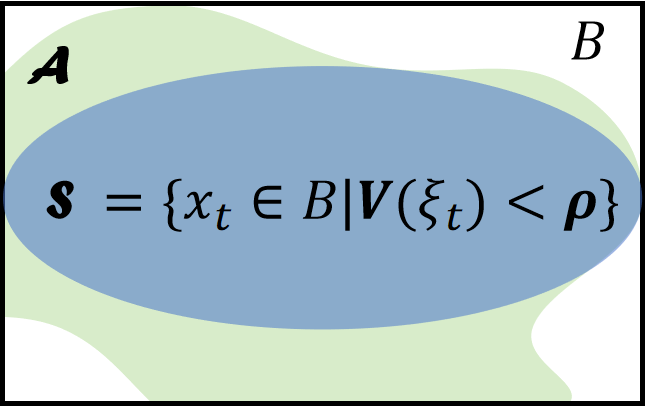
\includegraphics[width=0.45\textwidth]{figures/ROA.png}
%   \caption{The $\calB$ is the region of interest, 
%   $\calA$ is a non-covex region of attraction which is hard to be detected, 
%   and $\calS=\{\myvec{x}_{t}\in \calB | V(\myvec{\xi}_{t}) < \rho\}$ 
%   is the convex inner approximation of $\calA$, 
%   $V(\myvec{\xi}):\bbR^{n_{\myvec{\xi}}} \to \bbR$ 
%   is a lyapunov function and $\myvec{\xi}_{t} = [\myvec{x}_{t}, \myvec{e}_{t}]^{T}$.}\label{fig:roa}
%   \end{center}
%   \vskip -0.3in
% \end{figure*}

\begin{figure}[htbp]
    \centerline{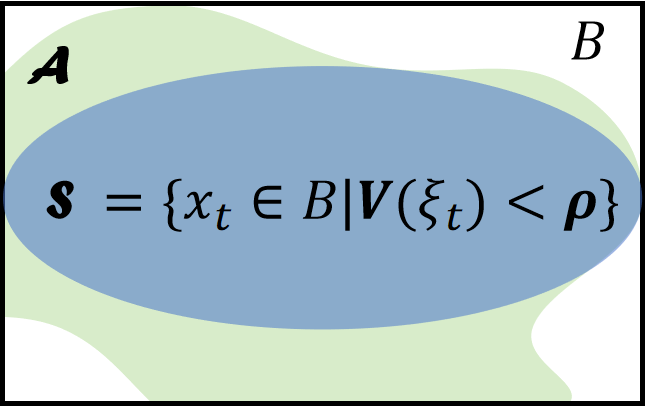
\includegraphics[width=0.8\columnwidth]{figures/ROA.png}}
    \caption{The $\calB$ is the region of interest, 
    $\calA$ is a non-covex region of attraction which is hard to be detected, 
    and $\calS=\{\myvec{x}_{t}\in \calB | V(\myvec{\xi}_{t}) < \rho\}$ 
    is the convex inner-approximation of $\calA$, 
    $V(\myvec{\xi}):\bbR^{n_{\myvec{\xi}}} \to \bbR$ 
    is a Lyapunov function and $\myvec{\xi}_{t} = [\myvec{x}_{t}, \myvec{e}_{t}]^{T}$. }
    % $\myvec{x}_0 \in \calA \textbackslash \calS$, its lower bound on minimum 
    % distortion cannot be directly determined by $\calS$. 
    \label{fig:roa}
\end{figure}

When the set of equilibrium states $\myvec{x}^{\star}$ 
in \roa secnario constitutes 
the target set TR as defined in \ra method, 
the \roa corresponds to the reach-avoid 
set as mentioned in \ra method. 
Fig.\ref{fig:roa} presents the relationships among the region of 
interest $\calB$, the region of attraction (\roa) $\calA$, 
and one of the potential inner approximations of $\calA$, 
denoted as $\calS$. 
If $\exists \myvec{x}_{t} \notin \calB,\ t\in \bbN$, 
then the initial state $\myvec{x}_{0}$ is deemed unsafe 
for the scenario. 
Since 
% the \roa is typically non-convex, 
identifying the precise region of $\calA$ is NP-hard. 
Verification studies 
% , therefore, aim to approximate the $\calA$ 
% by computing its convex inner 
% approximation $\calS$~
\cite{dai2021lyapunov,wu2023neural,yanglyapunov} 
inner-approximate $\calA$ 
through an optimization based on Lyapunov conditions~\cite{lyapunov1992general}:
\begin{subequations}
  \begin{align}
    max_{V} &Vol(\calS) \label{eq:lapunov optimization} \\
    s.t.&V(\myvec{\xi}_{t}) > 0\ \forall \myvec{\xi}_{t}\neq \myvec{\xi}^{\star}\in \calS \label{eq:lyapunov condition1} \\
    &V(\myvec{\xi}_{t+1}) - V(\myvec{\xi}_{t}) \leq -\kappa V(\myvec{\xi}_{t})\ \forall \myvec{\xi}_{t}\in \calS \label{eq:lyapunov condition2} \\
    &V(\myvec{\xi}^{\star}) = 0. \label{eq:lyapunov condition3}
  \end{align}
\end{subequations}
The $\kappa > 0$ is a set parameter for exponential 
stability convergence rate. Constrains (\ref{eq:lyapunov condition1}), 
(\ref{eq:lyapunov condition2}), and (\ref{eq:lyapunov condition3}) 
are the Lyapunov conditions, guarantee the states from $\calS$ 
lead system converge to the equilibrium state $\myvec{x}^{\star}$ 
and $\myvec{\xi}^{\star} = [\myvec{x}^{\star}, \myvec{0}_{n_{\myvec{x}}}]^{T}$. 
% As a result, the $\calS=\{\myvec{x}_{t}\in \calB | V(\myvec{\xi}_{t}) < \rho\}$ 
% from the optimization (\ref{eq:lapunov optimization}) 
% is the inner approximation of the \roa $\calA$. 
% The solution $V(\myvec{\xi}):\bbR^{n_{\myvec{\xi}}} \to \bbR$ 
% of optimization~(\ref{eq:lapunov optimization}) and a 
% threshold $\rho$ from optimization define the inner 
% approximation $\calS$ of the $\calA$ i.e., 
% $\calS=\{\myvec{x}_{t}\in \calB | V(\myvec{\xi}_{t}) < \rho\}$. 
The parameter $\rho$ is learned during the training of \nncs.
Additionally, the Lyapunov function 
$V(\myvec{\xi}):\bbR^{n_{\myvec{\xi}}} \to \bbR$ 
has following learnable structure:
\begin{equation}\label{eq:lapunov function}
  V(\myvec{\xi}_{t}) = 
  (\myvec{\xi}_{t} - \myvec{\xi}^{\star})^{T}
  (\epsilon \mymatrix{I} + \mymatrix{R}^{T}\mymatrix{R})
  (\myvec{\xi}_{t} - \myvec{\xi}^{\star}),
\end{equation}
The structure~(\ref{eq:lapunov function}) of $V(\myvec{\xi})$ 
naturally satisfies the Lyapunov conditions (\ref{eq:lyapunov condition1})
and (\ref{eq:lyapunov condition3}). 

% There is something that deserves to be noticed. 
% The $\myvec{x}_0 \in \calA \textbackslash \calS$ 's 
% lower bound on minimum 
% distortion cannot be directly determined by $\calS$. 
% Otherwise, our approach inner-approximates 
% $\lVert \myvec{x}_{0} - \myvec{z}_{0} \rVert$ 
% for $\myvec{z}_{0} \in \calA$. While utilizing the
% $\calS$ from barrier functions to 
% estimate the lower bound on minimum distortion, 
% $\myvec{z}_{0}\in \calS$ is inherently assumed. 
%%%%%%%%%%%%%%%%%%%%%%%%%%%%%%%%%%%%%%%%%%%%%%%%%%%%%%%%%%%%%%%%%%%%%%%%%%%%%%%%%%%%%%%%%%%%%%%%%%%%%%
\section{Robustness evaluation for \nncs}\label{sec:method}
In this section, we begin by providing 
the definition pertaining to minimum distortion and 
some lemmas. 
Subsequently, we conduct the lower bound on 
minimum distortion of \nncs by 
proving its Lipschitz continuity with 
respect to the initial state $\myvec{x}_{0}$, 
as delineated in Theorem~\ref{theorem:nncs Lipschitz continuity} 
and~\ref{theorem:Robustness evaluation for NNCS}, no matter in 
the \ra or \roa method. 
The conducted lower bound on the minimum 
distortion is remarked as robustness evaluation. 


\begin{definition}(Minimum distortion)\label{def:minimum distortion}
  Let $\myvec{x}_{0} \in \bbR^{n_{\myvec{x}}}$ is the initial 
  vector of $\nncs : \bbR^{n_{\myvec{x}}} \to \bbR^{n_{\myvec{y}}}$, 
  and $\myvec{x}_{0}\in \calA$. The 
  p-norm minimum distortion $\Delta_{p,min}$ for $\myvec{x}_{0}$ is denoted as the 
  smallest perturbation $\Delta_{p}= \lVert \delta \rVert_{p}$ s.t. 
  $\myvec{x}_{0}+\delta \notin \calA$. 
\end{definition}

However, identifying the precise 
region of $\calA$ for the precise $\Delta_{p,min}$, 
poses a significant challenge as it is a NP-hard problem. 
Our robustness evaluation computed as the 
lower bound on $\Delta_{p,min}$, 
denoted as $\Delta_{p,min}^{L}= \lVert 
  \delta_{min}^{L} \rVert_{p}$, 
such that the perturbed state $\myvec{z}_{t}=
f_{d}^{(t)}(\myvec{x}_{0}+
\delta_{min}^{L}) \notin \calS$ within a finite time $t$ 
and $\myvec{x}_{0} \in \calA$. 
Given that $\calS \subseteq \calA$, 
it follows that $\Delta_{p,min}^{L} \leq \Delta_{p,min}$, 
the $\Delta_{p,min}^{L}$ is the robustness evaluation in \ren. 
Before presenting the robustness evaluation, it is necessary 
to introduce several assumptions and lemmas.

\textbf{Assume 1}: 
Because both the dynamics $f(\myvec{x}, \myvec{y})$ 
and $h(\myvec{x})$ simulate the continuous dynamics of systems, 
it is a common assumption in various tasks such as 
stability analysis~\cite{chakraborty2011nonlinear,chen2014stability}, 
controller design~\cite{korda2014controller,mauroy2016global}, 
and robustness verification~\cite{wu2023neural,yanglyapunov} and so on. 
to consider the dynamics $f(\myvec{x}, \myvec{y})$ to be continuously 
differentiable with respect to $\myvec{x}$ and $\myvec{y}$, respectively, 
as is $h(\myvec{x})$ with respect to $\myvec{x}$.

\textbf{Assume 2}: 
For the convenience of the following proofs, 
assume that the neural networks $\phi_{\pi}$ and 
$\phi_{obs}$ have a pair of input-output layers, and 
only one hidden connected layer with common activation 
functions (like \relu, Leaky\relu, Sigmoid, Tanh and so on). 
% Additionally, we analyze the \nncs with activations 
% which are not absolutely Lipschitz continuous, like \relu or LeakyReLU. 

\begin{lemma}\label{lemma:CLEVER}
  According to the appendix C and D in 
  Weng et al.~\cite{weng2018evaluating}, 
  it is stated that a neural network $\phi(\myvec{x})$ 
  is continuously differentiable almost everywhere 
  with respect to its input $\myvec{x}$, 
  despite the activation functions used in the network 
  are not absolutely Lipschitz continuity (like \relu). 
  In other words, $\phi(\myvec{x})$ is Lipschitz continuous 
  almost everywhere with respect to $\myvec{x}$ i.e., 
  % The convex bounded closed input region $\calB$ can be split into limited pieces, 
  % denoted as $M_{0}, M_{1},\cdots,M_{m},\ m \in \bbN,\ m < \infty$. 
  % In each $M_{i},\ i \in [|m|]$, 
  let $\calB$ be a convex bounded closed input region, 
  $\phi(x):\calB \to \bbR$ be the neural network, 
  $\exists \ L_{q} > 0$, $\forall \myvec{x}, \myvec{y} \in \calB$, s.t.
  \begin{equation}
    \lVert \phi(\myvec{x}) - \phi(\myvec{y}) \rVert \leq
    L_{q}\cdot \lVert \myvec{x} - \myvec{y} \rVert_{p}
  \end{equation}
  where $\frac{1}{p} + \frac{1}{q} = 1$, $1 \leq p$ and $q \leq \infty$. 
  $L_{q} = max\{ || \nabla \phi(\myvec{x}) ||_{q}: \myvec{x} \in \bbB\}$, 
  $\nabla \phi(\myvec{x})$ is the gradient of $\phi(\myvec{x})$. 
\end{lemma}
% It is worthy to notice that in both $\phi_{\pi}(\myvec{x}, \myvec{y})$ 
% and $\phi_{obs}(\myvec{x}, \myvec{y})$, the input of networks 
% $[\myvec{x},\myvec{y}]^{T}$ is a 
% concatenated vectors of $\myvec{x}$ and $\myvec{y}$, which 
% is the input described 
% in Lemma~\ref{lemma:CLEVER}.

\begin{theorem}(Lipschitz continuity of barrier function 
    $g(\myvec{\xi})$)\label{theorem:nncs Lipschitz continuity}
    Given a \nncs considering the plant (\ref{eq:plant1}), 
    (\ref{eq:plant2}) within dynamics (\ref{eq:state_feedback_dynamic}) or 
    (\ref{eq:output_feedback_dynamic}), and the learned inner-approximation, 
    $\calS=\{\myvec{x}_{t}\in \calB | V(\myvec{\xi}_{t}) < \rho\}$. 
    The barrier function $g(\myvec{\xi}_{t}) = \rho - V(\myvec{\xi}_{t})$ 
    % constructed by (\ref{eq:lapunov function}) 
    is Lipschitz continuous almost everywhere with respect to the initial 
    input $\myvec{x}_{0}\in \calB$ within limited time steps $t$. 
    
\end{theorem}

Because of the differentiable continuous 
function $V(\myvec{x})$ in both \roa and \ra, 
the Theorem~\ref{theorem:nncs Lipschitz continuity} 
discusses the Lipschitz continuity of $\myvec{\xi}_{t}$ 
with respect to $\myvec{x}_{0}$ in fact, 
the Lipschitz constant of $V(\myvec{x})$ denoted as $L_{v}$. 
For convenience, we set $q=1$ and $p = \infty$ in the proof. 
As the output feedback secnario contains the state feedback one, 
the subsequent proofs will be directed towards the output feedback scenario. 

\begin{proof}\label{proof:nncs Lipschitz continuity}
    We employ the mathematical induction to establish the proof: 
  
    \textbf{Base case}: When $t = 0$, $\myvec{\xi}_{1} = 
    f_{d}(\myvec{\xi}_{0}) = [\myvec{x}_{1}, 
    \hat{\myvec{x}}_{1} - \myvec{x}_{1}]^{T}$, 
    let $\myvec{z}_{0}\in \calB$, $\myvec{z}_{0} \neq \myvec{x}_{0}$, 
    where $\tilde{\myvec{z}}_{0} = [\myvec{z}_{0}, \hat{\myvec{z}}_{0}]$, 
    and $\hat{\myvec{z}}_{0} = \mymatrix{H}\myvec{z}_{0}$, 
    $\hat{\myvec{z}}_{0}\in \bbR^{n_{\myvec{x}}}$, then: 
    \begin{equation}~\label{eq:nncs Lipschitz continuity 1}
      \begin{aligned}
        &||f_{d}(\tilde{\myvec{z}}_{1}) - f_{d}(\myvec{\xi}_{1})|| = 
        ||\begin{bmatrix}
          \myvec{z}_{1} - \myvec{x}_{1},\\ 
          \hat{\myvec{z}}_{1} - \hat{\myvec{x}}_{1} - (\myvec{z}_{1} - \myvec{x}_{1})
        \end{bmatrix}|| \\ 
        \leq& || \myvec{z}_{1} - \myvec{x}_{1} || + || \hat{\myvec{z}}_{1} - \hat{\myvec{x}}_{1}  - (\myvec{z}_{1} - \myvec{x}_{1})||\\
        % \leq&
        % \begin{bmatrix}
        %   ||f(\myvec{z}_{0}, \pi(\hat{\myvec{z}}_{0}, \myvec{h}(\myvec{z}_{0}))) - f(\myvec{x}_{0}, \pi(\hat{\myvec{x}}_{0}, \myvec{h}(\myvec{x}_{0})))||,\\ 
        %   \begin{aligned}
        %     &||f(\hat{\myvec{z}}_{0}, \pi(\hat{\myvec{z}}_{0}, \myvec{h}(\myvec{z}_{0}))) - f(\hat{\myvec{x}}_{0}, \pi(\hat{\myvec{x}}_{0}, \myvec{h}(\myvec{x}_{0})))|| 
        %     \\+&|| \phi_{obs}( \hat{\myvec{z}}_{0}, \myvec{h}(\myvec{z}_{0}) - \myvec{h}(\hat{\myvec{z}}_{0}) ) - 
        %     \phi_{obs}( \hat{\myvec{x}}_{0}, \myvec{h}(\myvec{x}_{0}) - \myvec{h}(\hat{\myvec{x}}_{0}) )||\\
        %      +&|| \phi_{obs}( \hat{\myvec{z}}_{0}, \myvec{0}_{n_{\myvec{y}}} ) - \phi_{obs}( \hat{\myvec{x}}_{0}, \myvec{0}_{n_{\myvec{y}}} ) || + 
        %      ||\myvec{z}_{0} - \myvec{x}_{0}| + |\myvec{z}_{1} - \myvec{x}_{1}||
        %   \end{aligned}
        % \end{bmatrix}
      \end{aligned}
    \end{equation}
    \begin{equation}~\label{eq:nncs Lipschitz continuity 1.1}
      ||\myvec{z}_{1} - \myvec{x}_{1}|| = ||f(\myvec{z}_{0}, \pi(\hat{\myvec{z}}_{0}, \myvec{h}(\myvec{z}_{0}))) - f(\myvec{x}_{0}, \pi(\hat{\myvec{x}}_{0}, \myvec{h}(\myvec{x}_{0})))||, 
    \end{equation}
    \begin{equation}~\label{eq:nncs Lipschitz continuity 1.2}
      \begin{aligned}
        &||\hat{\myvec{z}}_{1} - \hat{\myvec{x}}_{1}  - (\myvec{z}_{1} - \myvec{x}_{1})|| \leq ||\myvec{z}_{0} - \myvec{x}_{0}||+ ||\myvec{z}_{1} - \myvec{x}_{1}||\\
        +&||f(\hat{\myvec{z}}_{0}, \pi(\hat{\myvec{z}}_{0}, \myvec{h}(\myvec{z}_{0}))) - f(\hat{\myvec{x}}_{0}, \pi(\hat{\myvec{x}}_{0}, \myvec{h}(\myvec{x}_{0})))||
        \\+&|| \phi_{obs}( \hat{\myvec{z}}_{0}, \myvec{h}(\myvec{z}_{0}) - \myvec{h}(\hat{\myvec{z}}_{0}) ) - 
        \phi_{obs}( \hat{\myvec{x}}_{0}, \myvec{h}(\myvec{x}_{0}) - \myvec{h}(\hat{\myvec{x}}_{0}) )||\\
         +&|| \phi_{obs}( \hat{\myvec{z}}_{0}, \myvec{0}_{n_{\myvec{y}}} ) - \phi_{obs}( \hat{\myvec{x}}_{0}, \myvec{0}_{n_{\myvec{y}}} ) ||
      \end{aligned}
    \end{equation}
    Add $0 = -f(\myvec{x}_{0}, \pi(\hat{\myvec{z}}_{0},\myvec{h}(\myvec{z}_{0}))) + f(\myvec{x}_{0}, 
    \pi(\hat{\myvec{z}}_{0},\myvec{h}(\myvec{z}_{0})))$ 
    to $||f(\myvec{z}_{0}, \pi(\hat{\myvec{z}}_{0}, 
    \myvec{h}(\myvec{z}_{0}))) - f(\myvec{x}_{0}, \pi(\hat{\myvec{x}}_{0}, \myvec{h}(\myvec{x}_{0})))||$ 
    on the right side of the inequality~(\ref{eq:nncs Lipschitz continuity 1.2}). 
    Because of Assume 1, 
    let the Lipschitz constants of $f(\myvec{x},\myvec{y})$ 
    with respect to $\myvec{x}$, $\myvec{y}$ are 
    $L_{fx}$ and $L_{fy}$ respectively, then: 
    \begin{equation}~\label{eq:nncs Lipschitz continuity 2}
        \begin{aligned}
            ||\myvec{z}_{1} - \myvec{x}_{1}|| \leq& L_{fx}||\myvec{z}_{0} - \myvec{x}_{0}||_{\infty} + 
            L_{fy}||\pi(\hat{\myvec{z}}_{0}, \myvec{h}(\myvec{z}_{0})) - \\
            &\pi(\hat{\myvec{x}}_{0}, \myvec{h}(\myvec{x}_{0}))||_{\infty}
        \end{aligned}
    \end{equation}
    Because $\pi(\myvec{x}, \myvec{y})$ and 
    $\phi_{obs}(\myvec{x}, \myvec{y})$ are in the form of 
    $\myvec{W}_{2}\cdot \sigma ( \myvec{W}_{1}[:,:n_{\myvec{x}}]\cdot \myvec{x}
    + \myvec{W}_{1}[:,n_{\myvec{x}}:]\cdot \myvec{y} + \myvec{b}_{1})$ (Assume 2), 
    where $\myvec{W}_{i}$ and $\myvec{b}_{i}$ denote the weights and biases in 
    the i-th layer of neural networks, $\sigma(\cdot)$ implies the activation 
    functions. 
    % When treating $\myvec{x}$ (or $\myvec{y}$) 
    % as an independent variable, $\myvec{y}$ (or $\myvec{x}$) 
    % can be regarded as a constant. 
    According to Lemma~\ref{lemma:CLEVER}, 
    the Lipschitz constants of $\pi(\myvec{x}, \myvec{y})$ with respect to 
    $\myvec{x}$ and $\myvec{y}$ are denoted as $L_{\pi x}$ and $L_{\pi y}$, 
    likewise, $L_{\phi x}$ and $L_{\phi y}$ for $\phi_{obs}(\myvec{x}, \myvec{y})$. 
    Additionally, according to Assume 1 about $\myvec{h}(\myvec{x})$, the Lipschitz constant of $\myvec{h}(\myvec{x})$ with 
    respect to $\myvec{x}$ is denoted as $L_{h}$. As a result: 
    \begin{equation}~\label{eq:nncs Lipschitz continuity 3}
      ||\myvec{z}_{1} - \myvec{x}_{1}|| \leq
      L^{(0)}||\myvec{z}_{0} - \myvec{x}_{0}||_{\infty}
    \end{equation}
    where $L^{(0)} = (L_{fx} + L_{fy}\cdot L_{\pi x} + L_{fy}\cdot L_{\pi y}\cdot L_{h})$. 

    Emulate the process of (\ref{eq:nncs Lipschitz continuity 1}) 
    to (\ref{eq:nncs Lipschitz continuity 3}) through 
    Assume 1, 2, and Lemma~\ref{lemma:CLEVER}, we can obtain that: 
    \begin{equation}
      ||\hat{\myvec{z}}_{1} - \hat{\myvec{x}}_{1}|| \leq \hat{L}^{(0)}||\myvec{z}_{0} - \myvec{x}_{0}||_{\infty}
    \end{equation}
    where $\hat{L}^{(0)} = 
    (L_{fx} + L_{fy}\cdot L_{\pi x} + L_{fy}\cdot L_{\pi y}\cdot L_{h} + 2 L_{\phi y}\cdot L_{h} 
    + L_{\phi x} + L^{(0)})$. 
  
    Based on Eq.(\ref{eq:nncs Lipschitz continuity 1}), (\ref{eq:nncs Lipschitz continuity 2}), 
    and (\ref{eq:nncs Lipschitz continuity 3}), we obtain that: 
    \begin{equation}\label{eq:nncs Lipschitz continuity 4}
      ||f_{d}(\tilde{\myvec{z}}_{1}) - f_{d}(\myvec{\xi}_{1})|| 
      \leq (L^{(0)} + \hat{L}^{(0)})|| \myvec{z}_{0} - \myvec{x}_{0} ||_{\infty}
    \end{equation}
    It is naturally get: 
    \begin{equation}\label{eq:nncs Lipschitz continuity 5}
      ||g(\tilde{\myvec{z}}_{1}) - g(\myvec{\xi}_{1})|| 
      \leq L_{v}(L^{(0)} + \hat{L}^{(0)})|| \myvec{z}_{0} - \myvec{x}_{0} ||_{\infty}
    \end{equation}
  
    \textbf{Induction hypothesis}: When $t = \tau > 0$, assume that $\exists L^{(\tau)}$ 
    ,$\hat{L}^{(\tau)} > 0$ s.t. 
    \begin{subequations}
      \begin{align}
        &||\myvec{z}_{\tau} - \myvec{x}_{\tau}|| \leq L^{(\tau)}||\myvec{z}_{0} - \myvec{x}_{0}||_{\infty} \label{eq:nncs Lipschitz continuity 6}\\
        &||\hat{\myvec{z}}_{\tau} - \hat{\myvec{x}}_{\tau}|| \leq \hat{L}^{(\tau)}||\myvec{z}_{0} - \myvec{x}_{0}||_{\infty}\label{eq:nncs Lipschitz continuity 7}\\
        &||f_{d}(\tilde{\myvec{z}}_{\tau}) - f_{d}(\myvec{\xi}_{\tau})|| 
        \leq (L^{(\tau)} + \hat{L}^{(\tau)})|| \myvec{z}_{0} - \myvec{x}_{0} ||_{\infty}
      \end{align}
    \end{subequations}
  
    \textbf{Inductive step}: When $t = \tau + 1$, 
    \begin{equation}~\label{eq:nncs Lipschitz continuity 8}
      \begin{aligned}
        &||f_{d}(\tilde{\myvec{z}}_{\tau + 1}) - f_{d}(\myvec{\xi}_{\tau+1})|| = \\
        &||\begin{bmatrix}
          \myvec{z}_{\tau +1} - \myvec{x}_{\tau + 1},\\ 
          \hat{\myvec{z}}_{\tau + 1} - \hat{\myvec{x}}_{\tau + 1} - (\myvec{z}_{\tau + 1} - \myvec{x}_{\tau + 1})
        \end{bmatrix}||, \\ 
        \leq& || \myvec{z}_{\tau +1} - \myvec{x}_{\tau +1} || + || \hat{\myvec{z}}_{\tau +1} - \hat{\myvec{x}}_{\tau +1}  - (\myvec{z}_{\tau + 1} - \myvec{x}_{\tau + 1})||\\
      \end{aligned}
    \end{equation}
    As the same process as the Eq.(\ref{eq:nncs Lipschitz continuity 2}) to (\ref{eq:nncs Lipschitz continuity 4}), we have: 
    \begin{subequations}
      \begin{align}
        &||\myvec{z}_{\tau + 1} - \myvec{x}_{\tau + 1}|| \leq L||\myvec{z}_{\tau} - \myvec{x}_{\tau}||_{\infty}, \label{eq:nncs Lipschitz continuity 9}\\
        &||\hat{\myvec{z}}_{\tau + 1} - \hat{\myvec{x}}_{\tau + 1}|| \leq \hat{L}||\myvec{z}_{\tau} - \myvec{x}_{\tau}||_{\infty}\label{eq:nncs Lipschitz continuity 10}
      \end{align}
    \end{subequations}
    where $L = (L_{fx} + L_{fy}\cdot L_{\pi x} + L_{fy}\cdot L_{\pi y}\cdot L_{h})$, 
    $\hat{L} = 
    (L_{fx} + L_{fy}\cdot L_{\pi x} + L_{fy}\cdot L_{\pi y}\cdot L_{h} + 2 L_{\phi y}\cdot L_{h} 
    + L_{\phi x} + L)$, because of induction (\ref{eq:nncs Lipschitz continuity 6}) and (\ref{eq:nncs Lipschitz continuity 7}), 
    $\exists L^{(\tau + 1)},\ \hat{L}^{(\tau + 1)} > 0$, s.t. 
    \begin{equation}\label{eq:nncs Lipschitz continuity 11}
      ||g(\tilde{\myvec{z}}_{\tau + 1}) - g(\myvec{\xi}_{\tau + 1})|| 
        \leq L_{v}(L^{(\tau + 1)} + \hat{L}^{(\tau + 1)})|| \myvec{z}_{0} - \myvec{x}_{0} ||_{\infty}
    \end{equation}
    where $L^{(\tau + 1)} = L\cdot L^{(\tau)}$, $\hat{L}^{(\tau + 1)} = \hat{L}\cdot \hat{L}^{(\tau)}$. 
  
    In conclusion, $\exists L^{(t)},\ \hat{L}^{(t)}, L_{v} > 0$, $\forall t \in \bbN,\ \myvec{x}_{0}$, $\myvec{z}_{0}\in \calB$, 
    s.t. $||g(\tilde{\myvec{z}}_{t}) - g(\myvec{\xi}_{t})|| 
        \leq L_{v}(L^{(t)} + \hat{L}^{(t)})|| \myvec{z}_{0} - \myvec{x}_{0} ||_{\infty}$. 
  
\end{proof}

\begin{theorem}(Robustness evaluation for \nncs)\label{theorem:Robustness evaluation for NNCS}
    Given a p-norm ball 
    $\bbB_{p}(\myvec{x}_{0},\delta) = \{ \myvec{x}\in \calA | 
    \lVert \myvec{x} - \myvec{x}_{0} \rVert_{p} \leq \delta \}$, 
    the \nncs in Theorem~\ref{theorem:nncs Lipschitz continuity}, 
    barrier function $g(\myvec{\xi}_{t}) = \rho - V(\myvec{\xi}_{t})$ 
    within limited time steps $t$, 
    $L_{q}$ is the Lipschitz constant of $g(\myvec{\xi}_{0})$ 
    with respect to $\myvec{x}_{0} \in \calA$. 
    If perturbation $\Delta_{p} = ||\delta||_{p}$ satisfies: 
    \begin{equation}\label{eq:Robustness evaluation for NNCS 1}
      ||\delta||_{p} \leq \frac{\rho - V(\myvec{\xi}_{t})}{L_q}, 
    \end{equation}
    then perturbed state $\myvec{z}_{t} = f_{d}^{(t)}(\myvec{z}_{0}) \in \calS$ holds ture, 
    where $\calS \subseteq \calA$, $\myvec{z}_{0}\in \bbB_{p}(\myvec{x}_{0},\delta)$. 
    The value of $\Delta_{p,min}^{L} 
    \leq min_{\myvec{z}_{0} \neq \myvec{x}_{0}} \frac{\rho - V(\myvec{\xi}_{t})}{L_q}$ 
    is the robustness evaluation in \ren. 
\end{theorem}

\begin{proof}\label{proof:Robustness evaluation for NNCS}
    Because of Theorem~\ref{theorem:nncs Lipschitz continuity}, $\exists L_{q} > 0$, s.t. 
    \begin{equation}\label{eq:Robustness evaluation for NNCS 2}
      |g(\tilde{\myvec{z}}_{t}) - g(\myvec{\xi}_{t})| = | V(\tilde{\myvec{z}}_{t}) - V(\myvec{\xi}_{t}) | 
      \leq L_{q} \cdot || \myvec{z}_{0} - \myvec{x}_{0} ||_{p}
    \end{equation}
    After decomposing the absolute value in (\ref{eq:Robustness evaluation for NNCS 2}), 
    we have:
    \begin{equation}\label{eq:Robustness evaluation for NNCS 3}
      -L_{q}|| \myvec{z}_{0} - \myvec{x}_{0} ||_{p} \leq
      V(\tilde{\myvec{z}}_{t}) - V(\myvec{\xi}_{t}) \leq 
      L_{q}|| \myvec{z}_{0} - \myvec{x}_{0} ||_{p}
    \end{equation}
    For $\myvec{z}_{t}\in \calS$ to be true, there must be 
    \begin{equation}\label{eq:Robustness evaluation for NNCS 4}
      V(\tilde{\myvec{z}}_{t}) \leq L_{q}|| \myvec{z}_{0} - \myvec{x}_{0} ||_{p} + V(\myvec{\xi}_{t}) 
      \leq \rho
    \end{equation}
    (\ref{eq:Robustness evaluation for NNCS 4}) implies the 
    (\ref{eq:Robustness evaluation for NNCS 1}) holds. 
    Because the distortion from (\ref{eq:Robustness evaluation for NNCS 1}) 
    ensures $\myvec{z}_{t} \in \calS$ and 
    $\calS \in \calA$, the distortion from \ref{eq:Robustness evaluation for NNCS 1} 
    is the $\Delta_{p,min}^{L}$. 
  \end{proof}

%%%%%%%%%%%%%%%%%%%%%%%%%%%%%%%%%%%%%%%%%%%%%%%%%%%%%%%%%%%%%%%%%%%%%%%%%%%%%%%%%%%%%%%
\section{\ren evaluation via different distributions}\label{sec:algorithm}
Recall Section~\ref{sec:method}, 
we demonstrated that the lower bound on minimum 
distortion, given by 
$min_{\myvec{z}_{0} \neq \myvec{x}_{0}} 
\frac{\rho - V(\myvec{\xi}_{t})}{L_q}$, 
is related to the value function 
$V(\myvec{\xi}_{t})$ and its maximum cross-Lipschitz 
constant $L_{q}$, 
as expressed in (\ref{eq:Robustness evaluation for NNCS 1}). 
The maximum $L_{q}$ can be determined using the 
expression $max_{\myvec{z}_{0}\in\bbB_{p}(\myvec{x}_{0},
\delta)}||\frac{V(\tilde{\myvec{z}}_{t})- 
V(\myvec{\xi}_{t})}{\myvec{z}_{0} - \myvec{x}_{0}}||_{q}$, 
which is detailed in (\ref{eq:nncs Lipschitz continuity 11}).
Obtaining the maximum value of $L_{q}$ 
within a norm ball for the larger-scale 
neural networks of interest poses a challenge. 
This is because it is hard for $L_{q}$ to be readily 
determined through a single backpropagation 
or exhaustive search~\cite{weng2018evaluating}. 

To compute $L_{q}$ in \ren, we initially sample a 
pure state $\myvec{x}_{0}\in \calA$ and satisfies  
$\rho - V(\myvec{\xi}_{t}) > 0$ as required by 
Equation~(\ref{eq:nncs Lipschitz continuity 11}), 
% Since \ren aims to determine the maximum perturbation 
% that remains $\myvec{z}_{t} \in \calS$ as 
% the lower bound on the minimum distortion, 
we proceed to sample a collection of $n$ perturbed states 
$\myvec{z}_{0}^{(i)} \in 
\bbB_{p}(\myvec{x}_{0}, \delta)$, 
where $i \in [|n|]$ and $\delta$ represents 
the prescribed perturbation radius. 
Subsequently, we compute the value of $L_{q}$ from 
the pure and perturbed samples. However, obtaining a 
reliable estimate of 
$max_{\myvec{z}_{0}\neq\myvec{x}_{0}}L_{q}$ necessitates 
a substantial 
number of samples, and it remains challenging to 
ascertain whether the estimated $L_{q}$ corresponds to 
the true maximum value.
Methods proposed by Wood$\&$Zhang~\cite{wood1996estimation} 
and Weng et al.~\cite{weng2018evaluating} 
suggest employing Extreme Value Theory to estimate the 
distribution of $L_{q}$, followed by maximum likelihood 
estimation to determine its value. Nonetheless, a 
prerequisite for the Extreme Value Theory 
is that the distribution of samples must be non-degenerate, 
a condition that is not always satisfied 
in the \nncs of interest, 
as demonstrated in Sec~\ref{exam:validation}.

In this section, we prove and establish 
that the Lipschitz constant proven in 
Theorem~\ref{theorem:nncs Lipschitz continuity} 
adhere to two distinct 
distributions contingent upon the time step $t$ 
in Sec~\ref{sec:esimate in two distributions}.  
Furthermore, we delineate an algorithm 
for \ren framework 
in Sec~\ref{algorithm}. 
% for computing 
% these evaluations via extreme value theory and 
% peak detection, tailored to each distribution. 

\subsection{Estimate $L_{q}$ via two different distributions}\label{sec:esimate in two distributions}

In Theorem \ref{theorem:different distributions}, 
we establish that the $L_{q}$ distribution adheres 
to two distinct forms: a non-degenerate cumulative 
distribution and a One-point distribution. 
Subsequently, we present the Fisher-Tippett-Gnedenko 
Theorem in Lemma \ref{lemma:mle} to facilitate the 
estimation of $max_{\myvec{z}_{0}\neq\myvec{x}_{0}}L_{q}$ under the non-degenerate 
cumulative distribution.

\begin{lemma}\label{lemma:differentiable}
    Given the \nncs, and 
    barrier function $g(\myvec{\xi}_{t}) = \rho - V(\myvec{\xi}_{t})$  
    in Theorem~\ref{theorem:nncs Lipschitz continuity}. 
    $g(\myvec{\xi}_{t})$ is differentiable almost everywhere 
    for $\myvec{x}_{0} \in \calB$, $\forall t \in \bbN$.  
\end{lemma}

\begin{proof}\label{proof:differentiable}
    Because of Assume 1,  
    it is only necessary to prove that 
    $\myvec{\xi}_{t+1} = f_{d}(\myvec{\xi}_{t})$ is differentiable almost everywhere 
    for $\myvec{x}_{0}$ i.e., the Jacobi matrix $\nabla_{\myvec{x}_{0}}\myvec{\xi}_{t+1}$ 
    exists almost everywhere. It further implies that 
    $\nabla_{\myvec{x}_{0}}\myvec{x}_{t+1}$ and 
    $\nabla_{\myvec{x}_{0}}\hat{\myvec{x}}_{t+1}$ exists almost everywhere. 
  
    \textbf{Base case}: When $t = 1$, 
    \begin{subequations}
      \begin{align}
      &\nabla_{\myvec{x}_{0}}\myvec{x}_{1} = \nabla_{\myvec{x}_{0}}f_{d} 
      + \nabla_{\pi}f_{d} \cdot 
      \nabla_{\myvec{x}_{0}}\pi(\hat{\myvec{x}}_{0}, \myvec{h}(\myvec{x}_{0})), \label{eq:differentiable 1}\\
      &\nabla_{\myvec{x}_{0}}\hat{\myvec{x}}_{1} = \nabla_{\hat{\myvec{x}}_{0}}f_{d} 
      \cdot \nabla_{\myvec{x}_{0}}\hat{\myvec{x}}_{0} + \nabla_{\pi}f_{d} \cdot 
      \nabla_{\myvec{x}_{0}}\pi(\hat{\myvec{x}}_{0}, \myvec{h}(\myvec{x}_{0})) \nonumber \\
      & + \nabla_{\myvec{x}_{0}}\phi_{obs} 
      (\hat{\myvec{x}}_{0}, \myvec{h}(\myvec{x}_{0}) - \myvec{h}(\hat{\myvec{x}}_{0}))
      - \nabla_{\myvec{x}_{0}}\phi_{obs} (\hat{\myvec{x}}_{0}, \myvec{0}_{n_{\myvec{y}}}). \label{eq:differentiable 2}
      \end{align}
    \end{subequations}
    
    The derivative of neural networks $\nabla_{\myvec{x}_{0}}\pi(\hat{\myvec{x}}_{0}, 
    \myvec{h}(\myvec{x}_{0}))$ has the form based on Assume 2: 
    \begin{equation}\label{eq:differentiable 2.5}
      \begin{aligned}
      &\nabla_{\myvec{x}_{0}}\pi(\hat{\myvec{x}}_{0},\myvec{h}(\myvec{x}_{0})) = 
      \mymatrix{W}_{\pi 2} \cdot II( \mymatrix{W}_{\pi 1}[:,:n_{\myvec{x}}]\hat{\myvec{x}}_{0} + \myvec{b}_{\pi 1} \\
      & + \mymatrix{W}_{\pi 1}[:,n_{\myvec{x}}:]\myvec{h}(\myvec{x}_{0}) )
      \cdot [ \mymatrix{W}^{T}_{\pi 1}[:,:n_{\myvec{x}}] \cdot \nabla_{\myvec{x}_{0}}\hat{\myvec{x}}_{0} \\
      &+ \mymatrix{W}^{T}_{\pi 1}[:,n_{\myvec{x}}:] \cdot \nabla_{\myvec{x}_{0}}h(\myvec{x}_{0}) ]
    \end{aligned}
    \end{equation}
    where $II(\myvec{x})$ is an univariate indicator function: 
    \begin{equation}\label{eq:indicator function}
      II(\myvec{x}) = \left\{
        \begin{split}
            1, & \ \text{if } \myvec{x} > 0, \\
            0, & \ \text{if } \myvec{x} \leq 0.
        \end{split}
        \right. 
    \end{equation}
    Based on the Appendix D in \cite{weng2018evaluating}, because the count of 
    \relu activation is limited, 
    $\nabla_{\myvec{x}_{0}}\pi(\hat{\myvec{x}}_{0},\myvec{h}(\myvec{x}_{0}))$ 
    exists almost everywhere in $\myvec{x}_{0} \in \calB$. 
    The derivative of neural networks $\nabla_{\myvec{x}_{0}}\phi_{obs}$ 
    has the similar form as (\ref{eq:differentiable 2.5}).
    Consequently, according to Lemma~\ref{lemma:CLEVER}, Assume 1, and $\hat{\myvec{x}}_{0} = \mymatrix{H}\myvec{x}_{0}$ 
    in \cite{lyapunov1992general}, the (\ref{eq:differentiable 1}) and (\ref{eq:differentiable 2}) exist almost everywhere 
    in $\myvec{x}_{0} \in \calB$ when time step $t = 1$. 
  
    \textbf{Induction hypothesis}: When $t = \tau$, $\tau > 0$, 
    assume that $\nabla_{\myvec{x}_{0}}\myvec{x}_{\tau}$ and 
    $\nabla_{\myvec{x}_{0}}\hat{\myvec{x}}_{\tau}$ exists almost everywhere  in $\myvec{x}_{0} \in \calB$.
  
    \textbf{Inductive step}: When $t = \tau + 1$, 
    \begin{subequations}
      \begin{align}
        &\nabla_{\myvec{x}_{0}}\myvec{x}_{\tau + 1} = (\nabla_{\myvec{x}_{\tau}}f_{d} 
        + \nabla_{\pi}f_{d} \cdot 
        \nabla_{\myvec{x}_{\tau}}\pi(\hat{\myvec{x}}_{\tau}, \myvec{h}(\myvec{x}_{\tau}))) 
        \cdot \nabla_{\myvec{x}_{0}}\myvec{x}_{\tau}, \label{eq:differentiable 3}\\
        &\nabla_{\myvec{x}_{0}}\hat{\myvec{x}}_{\tau + 1} = (\nabla_{\hat{\myvec{x}}_{\tau}}f_{d} 
        \cdot \nabla_{\myvec{x}_{\tau}}\hat{\myvec{x}}_{\tau} + \nabla_{\pi}f_{d} \cdot 
        \nabla_{\myvec{x}_{\tau}}\pi(\hat{\myvec{x}}_{\tau}, \myvec{h}(\myvec{x}_{\tau})) \nonumber \\
        & + \nabla_{\myvec{x}_{\tau}}\phi_{obs}
        (\hat{\myvec{x}}_{\tau}, \myvec{h}(\myvec{x}_{t}) - \myvec{h}(\hat{\myvec{x}}_{\tau}))\nonumber \\
        &- \nabla_{\myvec{x}_{\tau}}\phi_{obs}(\hat{\myvec{x}}_{\tau}, \myvec{0}_{n_{\myvec{y}}})) 
        \cdot \nabla_{\myvec{x}_{0}}\hat{\myvec{x}}_{\tau}. \label{eq:differentiable 4}
      \end{align}
    \end{subequations}
    According to Lemma~\ref{lemma:CLEVER}, Assume 1, \cite{lyapunov1992general}, and induction hypothesis, 
    the (\ref{eq:differentiable 3}) and (\ref{eq:differentiable 4}) exist almost everywhere in $\myvec{x}_{0} \in \calB$ 
    when time step $t = \tau + 1$. 
  
    In conclusion, $g(\myvec{\xi}_{t})$ is differentiable almost everywhere 
    for $\myvec{x}_{0} \in \calB$, $\forall t \in \bbN$. 
    % According to the Lyapunov function (\ref{eq:lapunov function}): 
    
    % \begin{equation}\label{eq:differentiable 5}
    %   \nabla_{\myvec{x}_{0}} g(\myvec{\xi}_{t}) = 
    %   2\mymatrix{R}^{T}\mymatrix{R}\myvec{\xi}_{t} \cdot \nabla_{\myvec{x}_{0}}\myvec{\xi}_{t}.
    % \end{equation}
    
\end{proof}

In the following, we mark the $\nabla_{\myvec{x}_{0}} g(\myvec{\xi}_{t})$ as 
$\nabla g(\myvec{\xi}_{t})$ for convenience. 

\begin{lemma}(\cite{ponce2007continuity})\label{lemma:differentiable continuity}
  If $f(x):\bbR^{n_{x}} \to \bbR$ is differentiable and continuous 
  with respect to $x$, then its first-order derivative 
  $f'(x)$ is continuous almost everywhere with respect to 
  $x$. 
\end{lemma}
Lemma~\ref{lemma:differentiable continuity} is proved based on 
Baire category theorem~\cite{de1963subcompactness} and 
Baire Class 1 functions~\cite{kechris1990classification} in real analysis. 

Suppose n sampled 
$  \{\nabla g(\tilde{\myvec{z}}_{t}^{(i)})\} = 
\{||\frac{g(\tilde{\myvec{z}}_{t}^{(i)}) - g(\myvec{\xi}_{t})}
{\myvec{z}_{0} - \myvec{x}_{0}}||_{q}\} 
= \{||\frac{V(\tilde{\myvec{z}}_{t}^{(i)}) - V(\myvec{\xi}_{t})}
{\myvec{z}_{0} - \myvec{x}_{0}}||_{q}\}$. Denote them 
as a sequence of independent and identically distributed (iid) 
random variables $Y^{(i)}_{t}$, $i \in [|n|]$. 
$F_{Y^{(i)}_{t}}(y) = P(Y^{(i)}_{t} < y)$ is the CDF of $Y^{(i)}_{t}$. 
The $Y_{t}$ is used when the property is satisfied by any $Y^{(i)}_{t}$. 
Notice that the sampled 
$\{\nabla g(\tilde{\myvec{z}}_{t}^{(i)})\}$ 
can be interpreted as 
$||\nabla g(\myvec{\xi}_{t})||_{p}$, which represents 
the p-norm of the gradient of 
the function 
$g(\myvec{\xi}_{t}) = \rho - V(\myvec{\xi}_{t})$ 
in following proofs.

\begin{theorem}\label{theorem:different distributions}
  Considering the \nncs and the barrier function 
  $g(\myvec{\xi}_{t}) = \rho - V(\myvec{\xi}_{t})$ as stated in 
  Theorem~\ref{theorem:nncs Lipschitz continuity}, 
  the behavior of the $||\nabla g(\myvec{\xi}_{t})||_{q}$, 
  $\myvec{x}_{0} \in \calA$, 
  varies depending on the convergence of $\myvec{\xi}_{t}$ 
  as $t$ is finite. 
  If the time step $t$ lead to $\lnot(\myvec{\xi}_{t} \to \myvec{\xi}^{\star})$, 
  $\forall \myvec{x}_{0} \in \calA$, 
  $||\nabla g(\myvec{\xi}_{t})||_{q}$ 
  follows a non-degenerate distribution function, 
  and it can be estimated using Maximum Likelihood Estimate (\mle). 
  Conversely, if convergence occurs, $||\nabla g(\myvec{\xi}_{t})||_{q}$ 
  adheres to a degenerate distribution function, precluding 
  the use of MLE for estimation.

  % $||g(\myvec{\tilde{\myvec{z}}}_{t})||_{p}$ 
  % , where $\myvec{z}_{0} \in \calA$, $\myvec{z}_{0} \in \bbB_{p}(\myvec{x}_{0},\delta)$, 
  % $\myvec{x}_{0}\in \calA$ is the pure sample without perturbation. 
\end{theorem}

\begin{proof}\label{proof:different distributions}
  At first, we prove that $||\nabla g(\myvec{\xi}_{t})||_{q}$ 
  follows a non-degenerate distribution function which is a 
  cumulative distribution function (CDF)~\cite{burr1942cumulative} 
  while $\lnot(\myvec{\xi}_{t} \to \myvec{\xi}^{\star})$. It implies that 
  the distribution function $F_{Y_{t}}(y)$ 
  should satisfy limit property, boundedness, right-continuity, and monotonicity. 

  \begin{itemize}
    \item \textbf{Limit property}: 
    The $V(\xi)$ 
    aheres to Lyapunov conditions 
    (\ref{eq:lyapunov condition1}) and 
    (\ref{eq:lyapunov condition3}) or 
    belongs to a polynomial ring with 
    respect to $\myvec{x}$ in a closed-loop domain. 
    % $0 \leq V(\myvec{\xi}_{t}) \leq V(\myvec{\xi}_{0}$), $\forall \ t\in \bbN$, $\myvec{x}_{0} 
    % \in \calA$. 
    All of the $\myvec{z}_{0} - \myvec{x}_{0}$ 
    in $\frac{V(\tilde{\myvec{z}}_{t})-V(\myvec{\xi}_{t})}
    {\myvec{z}_{0} - \myvec{x}_{0}}$ are knowable. 
    As a result, the limit property i.e., $lim_{y\to \infty}F_{Y_{t}}(y) = 1$ and 
    $lim_{y\to -\infty}F_{Y_{t}}(y) = 0$ hold with both 
    \roa and \ra barrier functions. 

    \item \textbf{Right-continuity}: 
    Because $\myvec{\xi}_{t}$ is differentiable and (Lipschitz) 
    continuous almost everywhere to $\myvec{x}_{0}$, 
    proved in Theorem~\ref{theorem:nncs Lipschitz continuity} 
    and Lemma~\ref{lemma:differentiable}, 
    $\nabla\myvec{\xi}_{t}$ is continuous almost everywhere (i.e., right-continuous) 
    to $\myvec{x}_{0}$ according to Lemma~\ref{lemma:differentiable continuity}. 
    Consequently, the right-continuity $F_{Y_{t}}(y) = lim_{h\to 0}F_{Y_{t}}(y + h)$ 
    holds under $\myvec{x}_{0} \in \calB$, $y \in \bbR$ in 
    limited time step $t$.  
    % It implies that we only need to prove the right-continuity of $\frac{d\myvec{\xi}_{t}}{d\myvec{x}_{0}}$ 
    % to guarantee the right-continuity of $||\nabla g(\myvec{\xi}_{t})||_{p}$. \\
    % \textbf{Base case}: 
    % When time step $t = 1$, 
    % due to the Lemma~\ref{lemma:differentiable continuity} 
    % and Assume 1, $\frac{df_{d}}{d\myvec{x}_{0}}$, 
    % $\frac{df_{d}}{d\pi}$, and $\frac{dh}{d\myvec{x}_{0}}$ are 
    % continuous almost everywhere with respect to $\myvec{x}_{0}$. 
    % Moreover, the formulation (\ref{eq:differentiable 2.5}) in Lemma~\ref{lemma:differentiable} 
    % implies that $\frac{d\pi}{d\myvec{x}_{0}}(\hat{\myvec{x}}_{0}, \myvec{h}(\myvec{x}_{0}))$, 
    % $\frac{d\phi_{obs}}{d\myvec{x}_{0}} 
    % (\hat{\myvec{x}}_{0}, \myvec{h}(\myvec{x}_{t}) - \myvec{h}(\hat{\myvec{x}}_{0}))$, 
    % and $\frac{d\phi_{obs}}{d\myvec{x}_{0}} (\hat{\myvec{x}}_{0}, \myvec{0}_{n_{\myvec{y}}})$ 
    % are right-continuous almost everywhere with respect to $\myvec{x}_{0}$. 
    % Consequently, the right-continuity $F_{Y_{0}}(y) = lim_{h\to 0}F_{Y_{0}}(y + h)$ 
    % almost everywhere holds under $\myvec{x}_{0} \in \calB$, $y \in \bbR$.  

    % \textbf{Induction hypothesis}: 
    % Assume that $F_{Y_{\tau}}(y) = lim_{h\to 0}F_{Y_{\tau}}(y + h)$ 
    % almost everywhere holds when $t = \tau > 1$ i.e. 
    % $||\nabla g(\myvec{\xi}_{\tau})||_{p}$ is right-continuous almost 
    % everywhere with respect to $\myvec{x}_{0} \in \calB$. 

    % \textbf{Inductive step}: 
    % In the formulation (\ref{eq:differentiable 3}) and (\ref{eq:differentiable 4}), 
    \item \textbf{Monotonicity}: 
    Because we have proven that $\nabla g(\myvec{\xi}_{t})$ is 
    continuous almost everywhere to $\myvec{x}_{0} \in \calB$, we can 
    divide the state space $\calB$ into limited $n$ pieces, marked as 
    $\calB_{i},\ i \in [|n|]$. In each of $\calB_{i}$, $\nabla g(\myvec{\xi}_{t})$ 
    is continuous to $\myvec{x}_{0}$. 
    The $P_{\calB_{i}}( Y_{t} < y_{1} )$ can be denoted as the value of 
    $Vol( \{ \myvec{x}_{0}| Y_{t} < y_{1},\ \myvec{x}_{0} \in \calB_{i} \} ) 
    / Vol(\calB)$, $Vol(S)$ is the volume of the set $S$. 
    Due to the continuity in $\calB_{i}$, there has: 
    % $Vol( \{ \myvec{x}_{0}| Y_{t} < y_{1},\ \myvec{x}_{0} \in \calB_{i} \} ) \\
    %  \leq Vol( \{ \myvec{x}_{0}| Y_{t} < y_{2},\ \myvec{x}_{0} \in \calB_{i} \} ), \ \forall y_{1}<y_{2}$, 
    \begin{equation}\label{eq:monotonicity 1}
        \begin{aligned}
            &Vol( \{ \myvec{x}_{0}| Y_{t} < y_{1},\ \myvec{x}_{0} \in \calB_{i} \} ) \\
            & \leq Vol( \{ \myvec{x}_{0}| Y_{t} < y_{2},\ \myvec{x}_{0} \in \calB_{i} \} ), \ \forall y_{1}<y_{2}
        \end{aligned}
    \end{equation}
    which indicates $P_{\calB_{i}}( Y_{t} < y_{1}) \leq 
    P_{\calB_{i}}( Y_{t} < y_{2}), 
    \ \forall y_{1}<y_{2}$. 
    Because $P( Y_{t} < y_{1}) = \sum_{i = 0}^{i = n}P_{\calB_{i}}( Y_{t} < y_{1})$, 
    then the monotonicity $P( Y_{t} < y_{1}) \leq P( Y_{t} < y_{2}), 
    \ \forall y_{1}<y_{2}$ holds. 
    \item \textbf{Boundedness}: 
    Since the Limit property, Right-continuity and Monotonicity hold, 
    the Boundedness can be derived by other three properties. 
  \end{itemize}

  When $\lnot(\myvec{\xi}_{t} \to \myvec{\xi}^{\star})$, 
  $F_{Y_{t}}(y) = P(Y_{t} < y)$ 
  satisfies  limit property, 
  boundedness, right-continuity, and
  monotonicity, then
  $||\nabla g(\myvec{\xi}_{t})||_{q}$ (or samples $Y_{t}$)
  follows a non-degenerate cumulative distribution function. 
  The value samples $Y_{t}$ can be evaluated by \mle 
  according to the Fisher-Tippett-Gnedenko Theorem~\cite{smith1990extreme}. 

  When the time step $t$ is large enough 
  to guarantee $\myvec{\xi}_{t} \to \myvec{\xi}^{\star}$, 
  the value of sampled 
  $Y_{t} = 
  ||\frac{V(\tilde{\myvec{z}}_{t})-V(\myvec{\xi}_{t})}{\myvec{z}_{0} - \myvec{x}_{0}}||_{q}$. 
  Because the time step $t$ ensures 
  $V(\tilde{\myvec{z}}_{t}) - V(\myvec{\xi}_{t})$ 
  converge to $0$, 
  $\myvec{z}_{0} \in \bbB_{p}(\myvec{x}_{0},\delta)$. 
  % (Lyapunov condition (\ref{eq:lyapunov condition3})). 
  However, the sampled finite value $\lVert \myvec{z}_{0} - \myvec{x}_{0} \rVert$ does not converge to $0$, 
  the value of $Y_{t}$ converge to $0$, which adheres to 
  an One-point distribution i.e., sampled $Y_{t}$ converges to a constant $c\in \bbR$. 
\end{proof}

We demonstrate that the $L_{q}$ distribution conforms to 
a non-degenerate cumulative distribution when the time 
step $t$ is insufficiently large. 
Consequently, $max_{\myvec{z}_{0}\neq\myvec{x}_{0}}L_{q}$ 
can be achieved through the application of extreme 
value theory, commonly referred to as the 
Fisher-Tippett-Gnedenko Theorem.

\begin{lemma}(Fisher-Tippett-Gnedenko Theorem~\cite{smith1990extreme})\label{lemma:mle}
  If there exists a sequence of pairs of real numbers 
  $(a_{n},b_{n})$ such that $a_{n}>0$ and 
  $lim_{n\to \infty}F_{Y}^{(n)} = G(y)$, 
  where $G(y)$ is a non-degenerate cumulative 
  distribution function, then $G$ must correspond 
  to one of the following types of CDFs: 
  \begin{equation*}
    \begin{aligned}
      &Gumbel\ class\ (Type\ I):\\ 
      &\ G(y) = exp\{
        -exp\{ -\frac{y-a_{W}}{b_{W}} \}
      \} \\
      &Frechet\ class\ (Type\ II):\\
      &\ G(y) = \left\{
        \begin{split}
            &0, \ \text{if } y < a_{W}, \\
            &exp\{ -\frac{y-a_{W}}{b_{W}} \}^{-c_{W}}, \ \text{if } y \geq a_{W}.
        \end{split}
        \right. \\
      &Reverse\ Weibull\ class\ (Type\ III):\\ 
      &\ G(y) = \left\{
        \begin{split}
            &exp\{ -\frac{y-a_{W}}{b_{W}} \}^{-c_{W}}, \ \text{if } y < a_{W}, \\
            &1, \ \text{if } y \geq a_{W}.
        \end{split}
        \right. 
    \end{aligned}
  \end{equation*}
  where $a_{W}\in \bbR$, $b_{W} > 0$, and $c_{W} > 0$ 
  are the location, scale, and shape parameter, respectively. 
\end{lemma}

Because the CDF of $L_{q} = ||\nabla g(\myvec{\xi})||_{q}$ 
is right-bounded, 
as proved in the limit property of 
Theorem~\ref{theorem:different distributions}, 
we postulate that $max_{\myvec{z}_{0}\neq\myvec{x}_{0}}L_{q}$ adheres 
to the Reverse Weibull class. This is because the CDF 
of the Reverse Weibull distribution also has 
a right endpoint, which corresponds to the extreme 
value. This extreme value represents the unknown local 
cross Lipschitz constant $max_{\myvec{z}_{0}\neq\myvec{x}_{0}}L_{q}$ 
that we aim to estimate in \ren.
When the time 
step $t$ is sufficiently large, all sampled $L_{q}$ 
converge to the same constant $c$ as they adhere to a 
One-point distribution. 

We can find that if a \nncs satisfies the Lemma~\ref{lemma:CLEVER}, 
\ref{lemma:differentiable}, \ref{lemma:differentiable continuity}, 
and Assume 1, 2, the lower bound on the minimum distortion for 
\nncs can be determined using the \ren framework. 
\subsection{Algorithm for \ren}\label{algorithm}

To estimate robustness evaluation of \ren and 
the $max_{\myvec{z}_{0}\neq \myvec{x}_{0}}L_{q}$ 
for \nncs, 
we provide the algorithm~\ref{algorithm REN}. 
Given a \nncs which satisfies Assume 1 and 2, 
the input state of interest region $\calB$, 
% a pure data $\myvec{x}_{0} \in \calA$ s.t. 
% $g(\myvec{\xi}_{t}) > 0$ in the setted time steps $t$, 
a K-S test confidence interval $\alpha$ to 
detect whether 
the $L_{q}$ adhere to a non-degenerate 
CDF or an One-point 
distribution, 
barrier function of \nncs, 
and the maximum 
perturbation $R$ with the norm 
ball $\bbB_{p}(\myvec{x}_{0},R)$. 


\begin{algorithm}[!h]
  \caption{Algorithm of \ren}
   \label{algorithm REN} 
\begin{algorithmic}[1]
  \STATE {\bfseries Input:} the \nncs 
  which satisfies Assume 1 and 2, 
  the input state of interest region $\calB$, 
  equilibrium state $\myvec{x}^{\star}$, 
  perturbation norm $p$, 
  K-S test confidence interval $\alpha$, 
  barrier function $g(\myvec{\xi}) = \rho - V(\myvec{\xi})$, 
  batch size $N_{b}$, number of samples per batch $N_{s}$, 
  and maximum perturbation $R$. 
  \STATE {\bfseries Output:} \ren robustness evaluation 
  $\mu \in \bbR^{+}$ which is the lower bound on the 
  minimum distortion. 

  \STATE  initialize:
  $K \leftarrow \{\emptyset\}$, $q \leftarrow \frac{p}{p-1}$ \label{code:initialize}
  \WHILE {$\myvec{x}_{0}$ is $\emptyset$ or $g(\myvec{\xi}_{t}) < 0$}
    \STATE uniform and ramdom select the pure sample: \\
          $\myvec{x}_{0} \in \calB$\label{code:pure sample}
  \ENDWHILE

  \IF{ $g(\myvec{\xi}_{0}) > 0$  }
    \STATE Inner-approximate the minimum distortion in $\calS$: \\ 
    $L \leftarrow \textbf{D}(\myvec{x}_{0}, g(\myvec{x}))$\label{code:distortion S1}
  \ELSE
    \STATE $L \leftarrow NaN$\label{code:distortion S2}
  \ENDIF

  \FOR {$i \leftarrow 1$ to $N_{b}$}
    \FOR {$k \leftarrow 1$ to $N_{s}$}
      \WHILE {$\myvec{z}_{0}^{(ik)}$ is $\emptyset$ or $g(\tilde{\myvec{z}}_{t}) < 0$}
        \STATE ramdom select the perturbed sample: \\
              $\myvec{z}_{0}^{(ik)} \in \bbB_{p}(\myvec{x}_{0},R)$\label{code:perturbed sample}
      \ENDWHILE
      
      \STATE compute robustness evaluations: \\
            $b_{ik} \leftarrow ||\nabla g(\tilde{\myvec{z}}_{t}^{(ik)})||_{q}$\label{code:sample calculation}

    \ENDFOR

  \STATE Compile maximum Lipschitz constant:\\
        $K \leftarrow K \cup \{max\{max_{k}\{ b_{ik} \}, L\}\}$\label{code:maximum batch}
  \ENDFOR

  \IF{ $ks\_test$($K$) $\geq \alpha$ }
  \STATE $\hat{a}_{W} \leftarrow$ \mle $a_{W}$ in Type III distribution on $K$\label{code:Reverse Weibull}
  \ELSE
  \STATE $\hat{a}_{W} \leftarrow $ peak detection on $K$\label{code:one-point}
  \ENDIF

  \STATE $\mu \leftarrow min(\frac{g(\myvec{\xi}_{t})}{\hat{a}_{W}}, R)$\label{code:robustness evaluation}
\end{algorithmic}
\end{algorithm}
We initially generate $N_{b}$ batches 
of perturbed states. 
Within each batch, we sample $N_{s}$ instances of 
$\myvec{z}_{0}$. 
Uniformly and randomly select a pure data 
$\myvec{x}_{0} \in \calA$ within 
$g(\myvec{\xi}_{t}) > 0$ 
in the set time steps $t$ (line \ref{code:pure sample}). 
For the initial state $\myvec{x}_{0}$, 
if $\myvec{x}_{0} \in \calS$, we compute the minimum distance 
between $\myvec{x}_{0}$ and barrier function $g(\myvec{x})$ 
by optimization 
(line \ref{code:distortion S1} to \ref{code:distortion S2}). 
To ensure that 
$\myvec{z}_{t} \in \calS$, 
we check the condition 
$g(\tilde{\myvec{z}}_{t}) < 0$. 
If this condition is not met, the perturbed sample is 
resampled (line~\ref{code:perturbed sample}). 
Subsequently, we compute 
$||\nabla g(\tilde{\myvec{z}}_{t}^{(ik)})||_{q}$ 
according to distinct distributions. 
The sampled $L_q = ||\nabla 
g(\tilde{\myvec{z}}_{t}^{(ik)})||_{q}$ 
is calculated as a candidate 
maximum Lipschitz constant in 
line~\ref{code:sample calculation}. 
Subsequently, we extract the maximum value from 
the candidates in line \ref{code:maximum batch}. 
Thereafter, if the $N_b$ sampled Lipschitz constants in $K$ 
adhere to Reverse Weibull contribution, the result 
of K-S is more than $\alpha$. 
We perform maximum likelihood 
estimation of the Reverse Weibull distribution 
parameters, with the location parameter 
$\hat{a}_{W}$ serving as a potential estimate 
for $max_{\myvec{z}_{0}\neq\myvec{x}_{0}}L_{q}$ 
(line~\ref{code:Reverse Weibull}). It is important to 
note that Lemma~\ref{lemma:mle} is applicable when 
the count of samples is sufficient. In cases 
where the number of samples is inadequate 
or the samples adhere to One-point contribution, 
we resort to peak detection 
(line~\ref{code:one-point}). 
Ultimately, we use 
the maximum $L_q$ to compute the robustness 
estimate in \ren (lines~\ref{code:robustness evaluation}). 
% Because we employ a uniform sampling and 
% consistently compile the maximum Lipschitz constant. 
% Consequently, the majority of the samples 
% conform to a single distribution, 
% alternating between the Reverse Weibull and 
% One-point distributions. 
Notably, there is no scenario where 
samples from two different distributions 
would be mixed together due to 
the line~\ref{code:maximum batch} Algorithm.\ref{algorithm REN}
% Notably, the Lipschitz 
% constant sampled from the Reverse Weibull distribution 
% is always greater than that of the 
% One-point distribution because of the Lyapunov conditions. 
%%%%%%%%%%%%%%%%%%%%%%%%%%%%%%%%%%%%%%%%%%%%%%%%%%%%%%%%%%%%%%%%%%%%%%%%%%%%%%%%%%%%%%%%%%%%%%%%%%%%%%
\section{Experiments}\label{sec:exp}

We develope a framework, 
termed Robustness Evaluation for \nncs (\ren), 
to estimate the lower bound 
of minimum distortion in \nncs. 
The existing studies on \roa provides 
a comprehensive setup for both the 
state and output secnarios, and is notably general. 
Consequently, our 
experiments mainly employ 
the models and scenarios derived 
from \roa studies~\cite{yanglyapunov}.
We first delineate the configurations in 
Exp~\ref{exam:configuration}. In Exp~\ref{exam:validation}, 
we demonstrate that the 
Reverse Weibull and the One-point distributions 
adequately fit the empirical distributions of the 
cross Lipschitz constant $L_{q}$. 
Subsequently, 
in Exp \ref{exam:efficiency}, 
we involve a difference experiment 
to distinguish the \ren robustness evaluation 
from the robustness 
evaluation computed by barrier functions. 
Finally, in Exp \ref{exam:comparison}, we compare the 
lower bound provided by \ren with the 
minimum distortions achieved by baselines 
to show the soundness and applications of \ren. 

% The code resources of \ren can be found on 
% \todo{U R L!!!}. 

% First, experiments are conducted 
% to corroborate the distribution 
% properties established by our work. 
% Subsequently, the experimental results 
% confirmed the observations regarding 
% the lower bound on minimum distortion 
% produced by barrier functions, thereby 
% substantiating that \ren framework is 
% different from the barrier functions. 
% Moreover, comparative experiments 
% are performed to assess the 
% lower bound on minimum distortion 
% among the \ren framework,  
% attack, and verification. 
% The results suggest that the \ren framework 
% can provide a sound lower bound on minimum 
% distortion that is applicable 
% in practice.

\subsection{Experiment Configurations}\label{exam:configuration}

\paragraph{Networks and tasks}

The assessment is carried out on three distinct tasks: 
pathtracking~\cite{snider2009automatic}, 
pendulum~\cite{mori1976control}, 
and 2D quadrotor~\cite{bouabdallah2007full}. 
These tasks are incorporated into VNN-COMP 
2024~\cite{brix2024fifth} as competitive scenarios 
for participants. 
All the \nncs come from \cite{yanglyapunov} 
with multiple activate functions. 
Their specifics are delineated in 
Table~\ref{table:NN_table}. 
The neurons and layer imply the number of neurons and 
layers in one time interval. As time step $t$ increases, 
so do the total neurons and layers of the whole \nncs. 
In the following experiments, all of the 
specifications such 
as state domain $\calB$ 
come from the spec.file in \cite{yanglyapunov}. 
Because \cite{yanglyapunov} contains that it is better 
to calculate $l_{\infty}$ norm ($p = \infty$) for 
PGD and \abcrown, we 
analysis the minimum distortion with $p = \infty$ in the 
following experiments. 
All samples use the same random seed. 

\paragraph{Baselines}
We employ iterative-based attack methodologies, 
projected gradient descent (PGD)~\cite{madry2017towards}, 
% Carlini $\&$ Wagner's attack (CW)~\cite{du2021fast}, 
% and iterative fast gradient sign method (I-FGSM)~\cite{goodfellow2014explaining}, 
alongside the SOTA network verifier \abcrown, 
to determine the minimum distortion of \nncs. 
% These methods serve as baselines in our experiments. 
Iterative-based attack techniques are predominantly 
designed for classification networks~\cite{madry2017towards,du2021fast}. 
% PGD is designed originally for classification NNs. 
In the \cite{yanglyapunov}, PGD is applied 
to the \nncs setting to generate adversarial examples 
for training. 
% Consequently, our work additionally 
% extends the application of CW to \nncs. 
The generability of abcrown 
leads to its use in 
conjunction with PGD in \cite{yanglyapunov} to 
identify adversarial examples 
within the \nncs domain. 
% It is important to highlight that the tools 
% utilized in this paper and in \cite{yanglyapunov} 
% integrate \abcrown with the BaB (Branch and Bound), 
% thereby ensuring the soundness 
% and completeness of the verificaiton, 
% despite the notable increase in computational time. 
The timeout settings are setted as 360000s for 
verification. 
The minimum distortion lower bound, 
computed via the barrier function 
associated with the inner-approximation $\calS\in \calA$, 
referred to the robustness evaluation $L$ 
for \nncs. Similarly, the one computed by 
Lipschitz constant proven in our work is referred to 
\ren robustness evaluation. 
% The iterations and learning rates 
% in all attack methods and \abcrown 
% are the same as 
% the PGD and \abcrown in \cite{yanglyapunov}, respectively. 

\paragraph{Machine and Software}
All experiments are conducted on a 
40-core 2.20GHz Intel Xeon Silver
4210 platform with 128GB memory and 
NVIDIA GeForce RTX 3090 platform 
with 24GB video memory. 
\ren is implemented in Python~3.10. 

\begin{table}[ht]
  \caption{Models used in the experiments.
  All the models are trained through PGD~\cite{madry2017towards}
  and \abcrown~\cite{wang2021beta} based on Lyapunov conditions. 
  The Neurons and Layers imply 
  the number of neurons and 
  layers in one time interval. 
  The terms "-state" or "-output" in Model 
  denotes that the scenario of the task involves 
  state feedback or output feedback. 
  The 'small' means that the \nncs is trained with 
  a small torque. }
  \label{table:NN_table}
     \vspace{-1em}
  \begin{center}\small
%%     \begin{small}
      % \begin{sc}
        \setlength{\tabcolsep}{0.4em}{
          \begin{tabular}{lrc}
            \toprule
             Model    & Neurons & Layers  \\
            \midrule
                    Pathtracking-state   & 51   & 5        \\
                    Pathtracking-state(small)   & 51   & 5        \\
            \midrule
                    Pendulum-state      & 51  & 5        \\
                    Pendulum-state(small)      & 51  & 5        \\
                    Pendulum-output      & 73   & 8        \\
                    % Pendulum-output(small)      & 73   & 8        \\
            \midrule

                    Quadrotor2d-state      & 24  & 3      \\
                    Quadrotor2d-output          & 54  & 6    \\
            \bottomrule
          \end{tabular}}
      % \end{sc}
%%     \end{small}
  \end{center}

\end{table}

%%%%%%%%%%%%%%%%%%%%%%%%%%%%%%%%%%%%%%%%%%%%%%%%%%%%%%%%%%%%%%%%%%%
\subsection{Validation of distinct distributions}\label{exam:validation}

To validate Reverse Weibull and the One-point distributions 
adequately fit the empirical distributions of the 
cross Lipschitz constant $L_{q}$ 
based on various value of $t$, 
we conduct 
Kolmogorov-Smirnov goodness-of-fit test 
(K-S test \cite{massey1951kolmogorov}) 
to estimate the fittness through p-values 
based on various batch size $N_b$, 
number of samples per batch $N_s$, and 
time step $t$. 
The time interval is $0.05$ second as 
the same as the one in Yang et al.~\cite{yanglyapunov}. 
If $p\_value \geq \alpha$, $\alpha = 0.95$, 
the Reverse Weibull distribution 
hypothesis cannot be rejected. 
Conversely, it implies that almost of the samples 
adhere to One-point distribution. 
The Fig~\ref{fig:experiment1.1} shows the 
results of K-S test in pathtracking within various 
$N_b$, $N_s$, and the constant $t$. 
Specifically, Figures (a), (b), and (c) 
display the K-S test results for samples with 
various $N_b \times N_s$ 
($500\times 100$, $500\times 500$, and 
$1000\times 100$). 
\begin{figure}[htbp]
  \centering
  % 第一个子图
  \begin{subfigure}[b]{0.15\textwidth}
    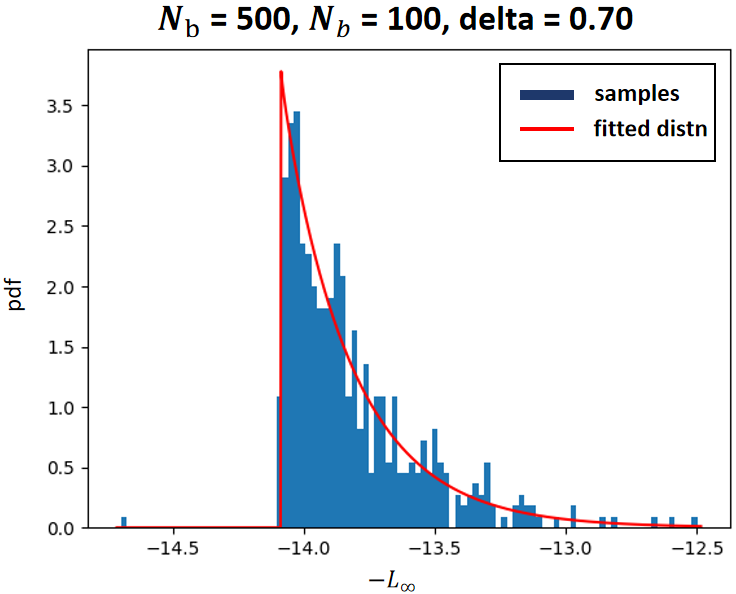
\includegraphics[width=\textwidth]
    {figures/experiment 1/pathtracking/pathtrack 500x100 10step}
    \caption{}
  \end{subfigure}
  % 第二个子图
  \begin{subfigure}[b]{0.15\textwidth}
    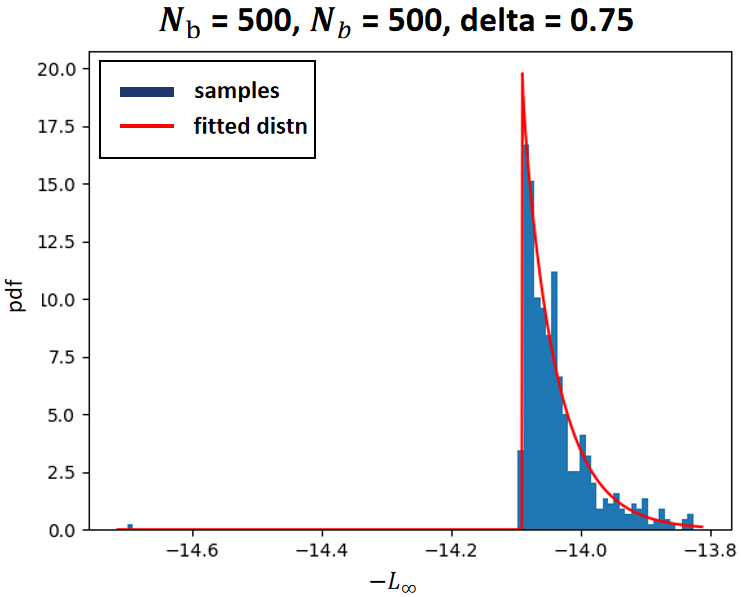
\includegraphics[width=\textwidth]
    {figures/experiment 1/pathtracking/pathtrack 500x500 10step}
    \caption{}
  \end{subfigure}
  % 第三个子图
  \begin{subfigure}[b]{0.15\textwidth}
    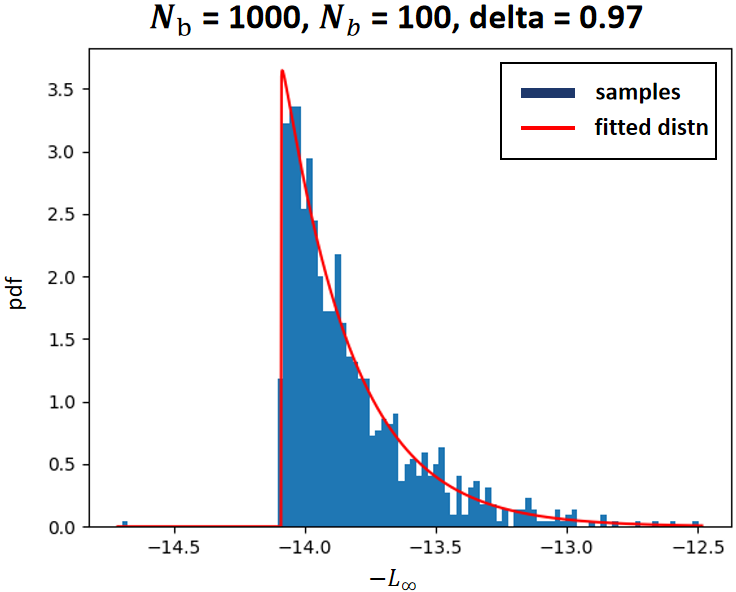
\includegraphics[width=\textwidth]
    {figures/experiment 1/pathtracking/pathtrack 1000x100 10step}
    \caption{}
  \end{subfigure}
  \caption{
  The cross Lipschitz constant sampled in the 
  pathtracking tasks, varying the batch size 
  ($N_b$), the number of samples per batch ($N_s$), 
  while maintaining a constant time step ($t = 10$). 
  The values of $N_b$, $N_s$, and p-values 
  (pVal) from K-S test 
  are presented atop each 
  subfigure. The blue parts represent 
  the empirical distribution of the Lipschitz 
  constants, whereas the red curve denotes the 
  theoretical Reverse Weibull distribution.  
  }
  \label{fig:experiment1.1}
\end{figure}


It should be noted that $t = 10$ was selected 
to ensure that the sampled states never 
converge to the equilibrium in pathtracking tasks. 
The figures indicate that as both 
$N_b$ and $N_s$ increase, the sampled $L_q$ values 
are more likely (pVal = 0.70, 0.75, and 0.97, 
respectively) to follow the Reverse 
Weibull distribution. 
This result supports 
the assumption stated in 
Lemma~\ref{lemma:mle}, which posits that 
the sample size must be sufficiently large. 
Furthermore, the analysis reveals that 
the effect of $N_b$ on the pVal is more 
pronounced than that of $N_s$. 
Consequently, to enhance the accuracy of 
the \ren while maintaining efficiency, we 
prefer to increasing in $N_b$ rather than $N_s$.

Figure~\ref{fig:experiment1.2} presents the 
K-S test for pathtracking as $t \in \{10, 100, 10000\}$, 
while keeping $N_b\times N_s = 1000\times 100$. 
Figure~\ref{fig:experiment1.2} (a) to (c) 
confirm Theorem~\ref{theorem:different distributions}, 
which posits that the number of time steps $t$ 
can alter the distribution of the Lipschitz 
constant in \nncs. As $t$ increases, the 
robustness evaluation (delta) also increases, 
indicating that \nncs 
exhibit greater robustness 
at larger $t$. 
This increased robustness is attributed to 
the ability of \nncs to partially rectify 
perturbations within each time interval. 
Otherwise, the result in PathTracking-state 
at $t = 10000$ also demonstrate the application 
of \ren on the 
large networks (about 510000 neruons).

\begin{figure}[htbp]
  \centering
  % 第一个子图
  \begin{subfigure}[b]{0.15\textwidth}
    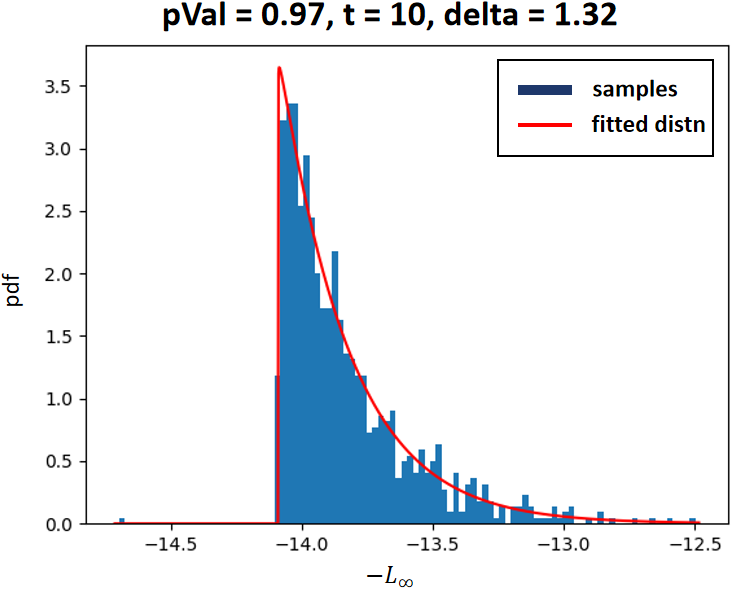
\includegraphics[width=\textwidth]
    {figures/experiment 1/pathtracking/pathtrack 1000x100 same t}
    \caption{}
  \end{subfigure}
  \hfill
  % 第二个子图
  \begin{subfigure}[b]{0.15\textwidth}
    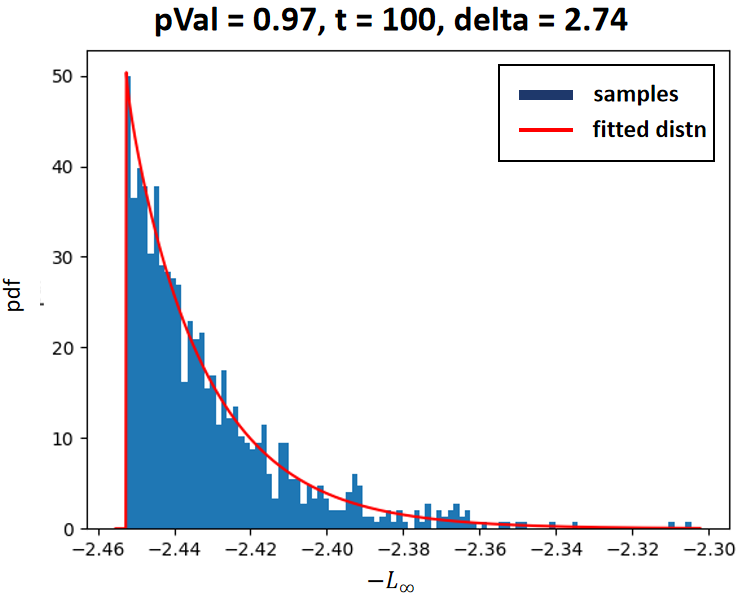
\includegraphics[width=\textwidth]
    {figures/experiment 1/pathtracking/pathtrack 1000x100 100step}
    \caption{}
  \end{subfigure}
  \hfill
  % 第三个子图
  \begin{subfigure}[b]{0.15\textwidth}
    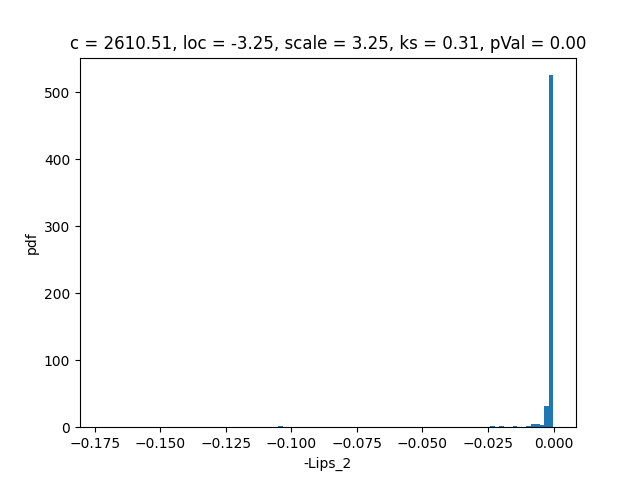
\includegraphics[width=\textwidth]
    {figures/experiment 1/pathtracking/pathtrack 1000x100 10000steps}
    \caption{}
  \end{subfigure}
  \caption{
  The cross Lipschitz constant sampled in the 
  pathtracking tasks, varying the time step $t$, 
  while maintaining a constant $N_b\times N_s$. 
  The values of $t$, the p-values 
  (pVal) from K-S test, and 
  robustness evaluation of \ren (delta) 
  are presented atop each 
  subfigure. 
}
  \label{fig:experiment1.2}
\end{figure}

% Figure~\todo{figure} shows the percentage of samples whose 
% distributions adhere to Reverse Weibull distribution or 
% One-point distribution through KS-test within 
% $\alpha = 0.95$, norm $p = \infty$. 
% The results show that all the samples in each tast 
% are close to $1oo\%$ fit the two distributions. 
% These samples are used in the following experiments. 

% Cpation of figure: The percentage of samples whose 
% distributions adhere to Reverse Weibull distribution or 
% One-point distribution. 
%%%%%%%%%%%%%%%%%%%%%%%%%%%%%%%%%%%%%%%%%%%%%%%%%%%
%%%%%%%%%%%%%%%%%%%%%%%%%%%%%%%%%%%%%%%%%%%%%%%%%%%
\subsection{Comparison between robustness evaluation from \ren and barrier functions}\label{exam:efficiency}
To differentiate the \ren robustness evaluation 
from that computed via barrier functions, 
we compare the lower bounds of minimum distortion 
they produce among 100 samples 
in Figure~\ref{fig:experiment2}, 
which displays cloudpoint images.
The cloudpoint figures (a) to (e) correspond to 
Pathtracking-state, Pendulum-state, 
Pendulum-output, Quadrotor2d-state, and 
Quadrotor2d-output, respectively. 
Red points represent the $L$ robustness 
evaluation, while blue points denote 
the \ren robustness evaluation. The horizontal 
axis indexes the samples, and the vertical 
axis denotes the lower bound on the 
minimum distortion.
\begin{figure}[htbp]
  \centering
  % 第一个子图
  \begin{subfigure}[b]{0.15\textwidth}
    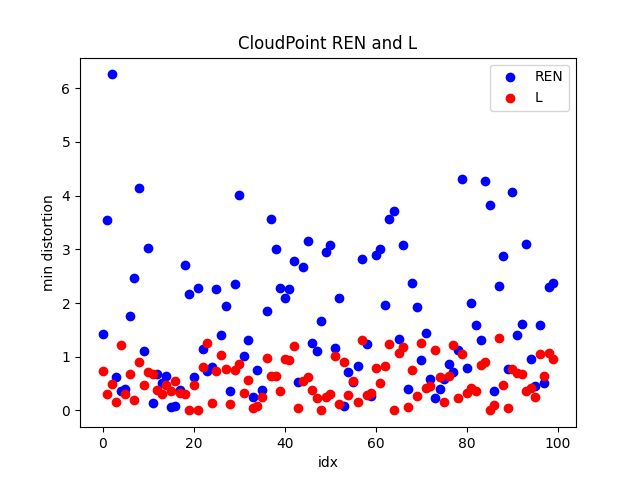
\includegraphics[width=\textwidth]
    {figures/experiment 2/pathtrack}
    \caption{}
  \end{subfigure}
  \hfill
  % 第二个子图
  \begin{subfigure}[b]{0.15\textwidth}
    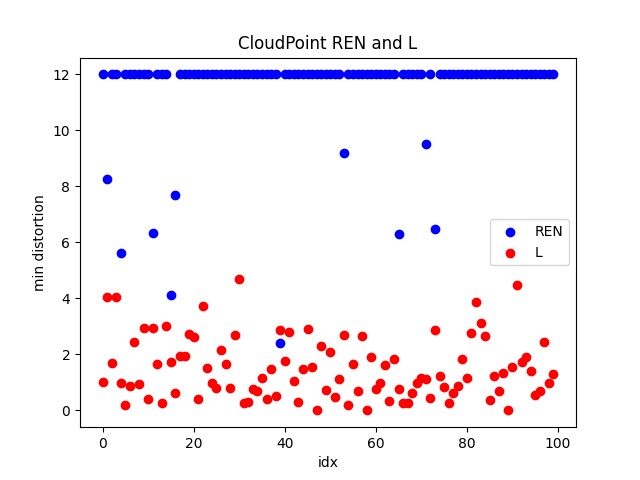
\includegraphics[width=\textwidth]
    {figures/experiment 2/pendulumstate}
    \caption{}
  \end{subfigure}
  \hfill
  % 第三个子图
  \begin{subfigure}[b]{0.15\textwidth}
    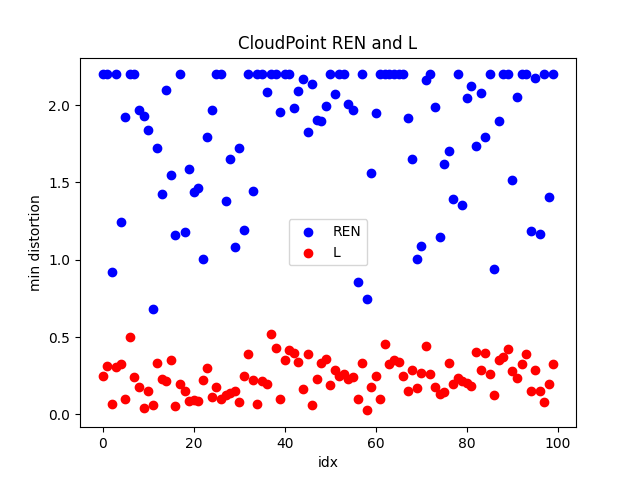
\includegraphics[width=\textwidth]
    {figures/experiment 2/pendulumout}
    \caption{}
  \end{subfigure}
  \newline
  % 调整第二行子图的水平间距
  \hspace*{\fill}
  % 第四个子图
  \begin{subfigure}[b]{0.15\textwidth}
    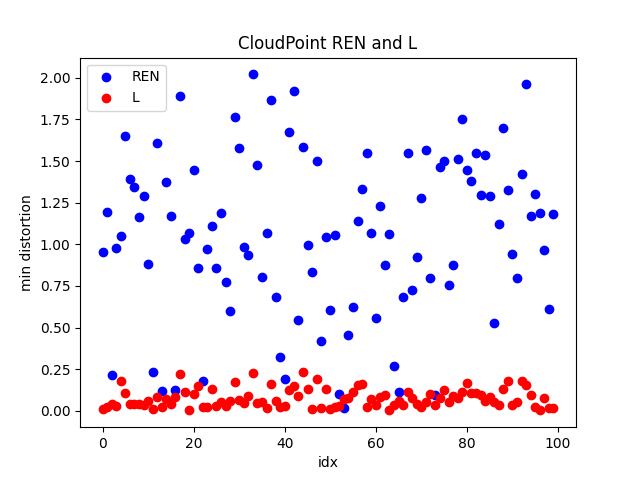
\includegraphics[width=\textwidth]{figures/experiment 2/Q2dstate}
    \caption{}
  \end{subfigure}
  \hspace{15pt} % 增加或减少这个值来调整间距
  % 第五个子图
  \begin{subfigure}[b]{0.15\textwidth}
    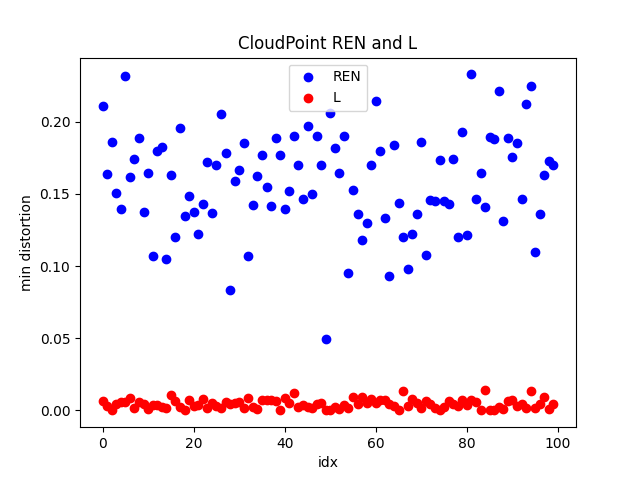
\includegraphics[width=\textwidth]{figures/experiment 2/Q2dout}
    \caption{}
  \end{subfigure}
  \hspace*{\fill}
  \caption{
  Both \ren and $L$ robustness evaluations 
  are derived from the same set of 100 samples. 
  Red points represent the $L$ robustness 
  evaluation, while blue points denote 
  the \ren robustness evaluation. The horizontal 
  axis indexes the samples, and the vertical 
  axis denotes the lower bound on the 
  minimum distortion.
}\label{fig:experiment2}
  
\end{figure}

In Figure~\ref{fig:experiment2}, the \ren robustness 
evaluation is observed to outperform the $L$ 
robustness evaluation across the majority of 
tasks. Specifically, the \ren robustness evaluation 
exceeds the $L$ robustness evaluation for 
97, 99, 100, 99, and 100 samples, respectively, 
in each task.
Notably, barrier functions were unable 
to handle 3 samples in the Pathtracking-state task. 
% We anticipate that this number may increase 
% as the number of samples grows. 
One reason for this difference is that the 
state considered in the $L$ robustness evaluation 
is limited to the barrier function corresponding 
to the inner-approximation, 
as opposed to the \ra or \roa region 
which is considered in the \ren robustness 
evaluation. Another reason is the difference 
in discussed perturbed sample $\myvec{z}_{0}$ 
in $\lVert \myvec{z}_{0} - \myvec{x}_{0} \rVert$. 
Specifically, the $L$ robustness evaluation 
focuses on $\myvec{z}_{0}$ 
in the inner-approximations 
from barrier functions, 
whereas the \ren robustness evaluation 
considers $\myvec{z}_{t}$ in the inner-approximation
while $\myvec{z}_{0}$ lies in the exact \ra 
or \roa. 

The experimental results indicate that the 
\ren robustness evaluation outperforms the $L$ 
robustness evaluation in the majority of 
tasks for \nncs. To enhance the tightness 
of the robustness evaluation provided 
by the \ren framework, we propose a combination 
of \ren with the $L$ robustness evaluation, 
as detailed in Algorithm~\ref{algorithm REN}.


%%%%%%%%%%%%%%%%%%%%%%%%%%%%%%%%%%%%%% 
\subsection{Comparison among \ren, verification, and attack }\label{exam:comparison}

In this study, we compare \ren framework 
in algorithm~\ref{algorithm REN}
against the minimal distortions attained 
by the baseline methods with time step $t = 10$ 
among the same 100 samples. 
Table~\ref{table:comparison} facilitates a 
comparative analysis of 
average $l_{\infty}$ distortions 
detected by the PGD, PGD[\ren] and \abcrown relative to 
\ren robustness evaluations. 
PGD[\ren] refers to the PGD within the 
\ren framework to reduce its detection 
domain for identifying adversarial examples. 
We determine that the lower 
bound on minimum distortion corresponds 
to the maximum potential perturbation 
for unsuccessful attack instances. 
To detect the precise minimum distortion 
through verification \abcrown as a standard, 
we utilize the dichotomy~\cite{jay1981gender} 
which is a typical method for detection. 
The dichotomy iteration and 
threshold are setted as $30$ and $1e^{-6}$, 
respectively, ensuring that 
the accuracy and efficiency of dichotomy. 
Term '-' means timeout issue. 

As anticipated by comparison with \abcrown, 
the results of attacks are 
regarded as the upper bound for 
the minimum distortion, 
our \ren framework establishes a sound 
lower bound on minimum distortion. 
\begin{table}[htbp]
    \caption{Comparisons on average \ren robustness evaluations 
    and distortions fonund by PGD, PGD[\ren] and \abcrown. The term '-' 
    means timeout issue. }
    \label{table:comparison}
    \begin{center}
      \begin{tabular}{|c|c|c|c|}
        \hline
        \textbf{Network} & Method & Time(s) & $\delta$\\
        \hline
        PathTracking-state & PGD & 15.608 & 2.250 \\
        & PGD[\ren] & - & 2.031 \\
        & \abcrown & 1.253k & 1.784 \\
        & \ren & 22.131 & 1.720 \\
        \hline
        PathTracking-state(small) & PGD & 15.608 & 2.250 \\
        & PGD[\ren] & - & 2.031 \\
        & \abcrown & 1.253k & 1.784 \\
        & \ren & 22.131 & 1.720 \\
        \hline
        Pendulum-state & PGD & 22.293 & 12.000 \\
        & PGD[\ren] & - & 12.000 \\
        & \abcrown & 2.731k & 12.000 \\
        & \ren & 23.951 & 11.459 \\
        \hline
        Pendulum-state(small) & PGD & 22.293 & 12.000 \\
        & PGD[\ren] & - & 12.000 \\
        & \abcrown & 2.731k & 12.000 \\
        & \ren & 23.951 & 11.459 \\
        \hline
        Pendulum-output & PGD & 48.659& 1.283 \\
        & PGD[\ren] & - & 1.007 \\
        & \abcrown & - & - \\
        & \ren & 33.586 & 0.341 \\
        % \hline
        % Pendulum-output(small) & PGD & 48.659& 1.283 \\
        % & PGD[\ren] & - & 1.007 \\
        % & \abcrown & - & - \\
        % & \ren & 33.586 & 0.341 \\
        \hline
        Quadrotor2d-state & PGD & 45.849 & 2.881 \\
        & PGD[\ren] & - & 2.093 \\
        & \abcrown & 3.085k & 1.363 \\        
        & \ren & 10.782 & 1.107 \\
        \hline
        Quadrotor2d-output & PGD & 57.631 & 0.450 \\
        & PGD[\ren] & - & 0.236 \\
        & \abcrown & - & - \\
        & \ren & 22.105 & 0.158 \\
        \hline
      \end{tabular}
    \end{center}
  \end{table}
% Furthermore, we find that the minimum distortions 
% for \nncs with observers are typically greater 
% than those for \nncs lacking observers. 
% This suggests that the observer serves is an effective 
% defenser, enhancing system robustness. 
%%%%%%%%%%%%%%%%%%%%%%%%%%%%%%%%%%%%%%%%%
In Table~\ref{table:comparison}, 
the robustness estimation identified by 
PGD[\ren] surpasses that of PGD by 
\todo{Number} on average. 
Specifically, all cases that are unsuccessfully 
attacked by PGD in \todo{Tasks}, 
obtaining the robustness evaluation as \todo{Number}. 
Meanwhile, the value evaluated 
by PGD[\ren] is \todo{Number} which is closer to 
the exact minimum distortion attained by \abcrown. 
The experimental findings 
suggest that the \ren framework can 
provide a lower bound for minimum distortion, 
thereby reducing the scope of search 
for attacks and increasing the possibility 
of detecting tighter adversarial examples. 
Although PGD[\ren] incurs an average 
time cost that is \todo{Number}\% 
higher than that of PGD, 
it consumes \todo{Number}\% less time on 
average compared to the total time of the \ren 
framework and PGD attack. This reduction 
in time is attributable 
to the decreased scope of the research, 
which facilitates the detection of 
adversarial examples in some cases, then 
attcak terminates earliy. 

Furthermore, torque is a critical parameter in the 
training of controller systems. Utilizing a 
small torque can augment the expressivity, 
convergence, and interpretability of systems. 
However, it may impact the robustness 
of systems~\cite{yanglyapunov}. 
Comparing \nncs with their versions 
trained with small torque, 
we observe that the lower bound on minimum 
distortion achieved by \ren in 
the PathTracking-state is \todo{Number} 
greater than that in the PathTracking-state(small). 
This finding aligns with the fact presented 
by Yang et al.~\cite{yanglyapunov}, 
which indicates that the $\calS$ 
in PathTracking-state encompasses 
the $\calS$ in PathTracking-state(small). 
The comparisons show the application 
of \ren framework 
on evaluation for \nncs. 

%%%%%%%%%%%%%%%%%%%%%%%%%%%%%%%%%%%%%%%%%
% save
Moreover, we find that verification methods 
encountered instances of failure. 
For example, the \abcrown reaches a 
timeout issue during the Quadrotor2d-output 
verification. This is because \abcrown invokes 
much more rounds of the gradient calculation 
of the \nncs than attacks, and more complex non-linear 
functions incur a higher computational cost, requiring more 
time to compute gradients and perform the verification. 

It is important to recognize the distinction 
in input requirements between \nncs equipped with observers 
and those without. For instance, 
while the inputs for the Quadrotor2d-state system 
encompass the quadrotor's complete position data, 
the inputs of Quadrotor2d-output system is limited to angle or 
lidar measurements, excluding location information which 
should be estimated by observers. 
This difference in inputs precludes a 
direct comparison of robustness using the 
minimum distortion of input between \nncs with and 
without observers.



%%%%%%%%%%%%%%%%%%%%%%%%%%%%%%%%%%%%%%%%%%%%%%%%%%%%%%%%%%%%%%%%%%%


\section{Conclusion}
\label{sec:conclusion}

This paper proposes a framework named \ren. 
Our work firstly determines one of the properties 
in Neural Network Controlled 
Systems (\nncs), its lower bound on 
minimum distortion, for all states of 
interest by leveraging the Lipschitz constants 
of \nncs. We establish the Lipschitz continuity 
of \nncs and investigate the different distributions 
adhered to by the Lipschitz constants. 
% The \ren robustness evaluation offers an 
% initial perturbation that closely approximates 
% the minimum distortion, which is utilized 
% by verification procedures to 
% estimate the robustness of the systems. 
Experimental results validate that the 
\ren framework provides the sound and 
sufficiently tight lower bound 
on minimum distortion for \nncs with theoretical 
guarantees and practical applicability. 
The \ren framework 
enables us to contemplate the training, 
evaluation, enhanced attak or defence, and other 
applications on \nncs, 
as well as the various 
ones on classification NNs, 
with \ren as a benchmark, 
in future works. 
We also hope for a mature dataset to 
standardize future works in \nncs, 
like MNIST and CIFAR-10 for 
classification NNs.
\clearpage
\bibliographystyle{./IEEEtran}
\bibliography{./IEEEexample}
\end{document}
%%%%%%%%%%%%%%%%%%%%%%%%%%%%%%%%%%%%%%%%%%%%%%%%%%
% \subsection{Maintaining the Integrity of the Specifications}

% The IEEEtran class file is used to format your paper and style the text. All margins, 
% column widths, line spaces, and text fonts are prescribed; please do not 
% alter them. You may note peculiarities. For example, the head margin
% measures proportionately more than is customary. This measurement 
% and others are deliberate, using specifications that anticipate your paper 
% as one part of the entire proceedings, and not as an independent document. 
% Please do not revise any of the current designations.

% \section{Prepare Your Paper Before Styling}
% Before you begin to format your paper, first write and save the content as a 
% separate text file. Complete all content and organizational editing before 
% formatting. Please note sections \ref{AA} to \ref{FAT} below for more information on 
% proofreading, spelling and grammar.

% Keep your text and graphic files separate until after the text has been 
% formatted and styled. Do not number text heads---{\LaTeX} will do that 
% for you.

% \subsection{Abbreviations and Acronyms}\label{AA}
% Define abbreviations and acronyms the first time they are used in the text, 
% even after they have been defined in the abstract. Abbreviations such as 
% IEEE, SI, MKS, CGS, ac, dc, and rms do not have to be defined. Do not use 
% abbreviations in the title or heads unless they are unavoidable.

% \subsection{Units}
% \begin{itemize}
% \item Use either SI (MKS) or CGS as primary units. (SI units are encouraged.) English units may be used as secondary units (in parentheses). An exception would be the use of English units as identifiers in trade, such as ``3.5-inch disk drive''.
% \item Avoid combining SI and CGS units, such as current in amperes and magnetic field in oersteds. This often leads to confusion because equations do not balance dimensionally. If you must use mixed units, clearly state the units for each quantity that you use in an equation.
% \item Do not mix complete spellings and abbreviations of units: ``Wb/m\textsuperscript{2}'' or ``webers per square meter'', not ``webers/m\textsuperscript{2}''. Spell out units when they appear in text: ``. . . a few henries'', not ``. . . a few H''.
% \item Use a zero before decimal points: ``0.25'', not ``.25''. Use ``cm\textsuperscript{3}'', not ``cc''.)
% \end{itemize}

% \subsection{Equations}
% Number equations consecutively. To make your 
% equations more compact, you may use the solidus (~/~), the exp function, or 
% appropriate exponents. Italicize Roman symbols for quantities and variables, 
% but not Greek symbols. Use a long dash rather than a hyphen for a minus 
% sign. Punctuate equations with commas or periods when they are part of a 
% sentence, as in:
% \begin{equation}
% a+b=\gamma\label{eq}
% \end{equation}

% Be sure that the 
% symbols in your equation have been defined before or immediately following 
% the equation. Use ``\eqref{eq}'', not ``Eq.~\eqref{eq}'' or ``equation \eqref{eq}'', except at 
% the beginning of a sentence: ``Equation \eqref{eq} is . . .''

% \subsection{\LaTeX-Specific Advice}

% Please use ``soft'' (e.g., \verb|\eqref{Eq}|) cross references instead
% of ``hard'' references (e.g., \verb|(1)|). That will make it possible
% to combine sections, add equations, or change the order of figures or
% citations without having to go through the file line by line.

% Please don't use the \verb|{eqnarray}| equation environment. Use
% \verb|{align}| or \verb|{IEEEeqnarray}| instead. The \verb|{eqnarray}|
% environment leaves unsightly spaces around relation symbols.

% Please note that the \verb|{subequations}| environment in {\LaTeX}
% will increment the main equation counter even when there are no
% equation numbers displayed. If you forget that, you might write an
% article in which the equation numbers skip from (17) to (20), causing
% the copy editors to wonder if you've discovered a new method of
% counting.

% {\BibTeX} does not work by magic. It doesn't get the bibliographic
% data from thin air but from .bib files. If you use {\BibTeX} to produce a
% bibliography you must send the .bib files. 

% {\LaTeX} can't read your mind. If you assign the same label to a
% subsubsection and a table, you might find that Table I has been cross
% referenced as Table IV-B3. 

% {\LaTeX} does not have precognitive abilities. If you put a
% \verb|\label| command before the command that updates the counter it's
% supposed to be using, the label will pick up the last counter to be
% cross referenced instead. In particular, a \verb|\label| command
% should not go before the caption of a figure or a table.

% Do not use \verb|\nonumber| inside the \verb|{array}| environment. It
% will not stop equation numbers inside \verb|{array}| (there won't be
% any anyway) and it might stop a wanted equation number in the
% surrounding equation.

% \subsection{Some Common Mistakes}\label{SCM}
% \begin{itemize}
% \item The word ``data'' is plural, not singular.
% \item The subscript for the permeability of vacuum $\mu_{0}$, and other common scientific constants, is zero with subscript formatting, not a lowercase letter ``o''.
% \item In American English, commas, semicolons, periods, question and exclamation marks are located within quotation marks only when a complete thought or name is cited, such as a title or full quotation. When quotation marks are used, instead of a bold or italic typeface, to highlight a word or phrase, punctuation should appear outside of the quotation marks. A parenthetical phrase or statement at the end of a sentence is punctuated outside of the closing parenthesis (like this). (A parenthetical sentence is punctuated within the parentheses.)
% \item A graph within a graph is an ``inset'', not an ``insert''. The word alternatively is preferred to the word ``alternately'' (unless you really mean something that alternates).
% \item Do not use the word ``essentially'' to mean ``approximately'' or ``effectively''.
% \item In your paper title, if the words ``that uses'' can accurately replace the word ``using'', capitalize the ``u''; if not, keep using lower-cased.
% \item Be aware of the different meanings of the homophones ``affect'' and ``effect'', ``complement'' and ``compliment'', ``discreet'' and ``discrete'', ``principal'' and ``principle''.
% \item Do not confuse ``imply'' and ``infer''.
% \item The prefix ``non'' is not a word; it should be joined to the word it modifies, usually without a hyphen.
% \item There is no period after the ``et'' in the Latin abbreviation ``et al.''.
% \item The abbreviation ``i.e.'' means ``that is'', and the abbreviation ``e.g.'' means ``for example''.
% \end{itemize}
% An excellent style manual for science writers is \cite{b7}.

% \subsection{Authors and Affiliations}\label{AAA}
% \textbf{The class file is designed for, but not limited to, six authors.} A 
% minimum of one author is required for all conference articles. Author names 
% should be listed starting from left to right and then moving down to the 
% next line. This is the author sequence that will be used in future citations 
% and by indexing services. Names should not be listed in columns nor group by 
% affiliation. Please keep your affiliations as succinct as possible (for 
% example, do not differentiate among departments of the same organization).

% \subsection{Identify the Headings}\label{ITH}
% Headings, or heads, are organizational devices that guide the reader through 
% your paper. There are two types: component heads and text heads.

% Component heads identify the different components of your paper and are not 
% topically subordinate to each other. Examples include Acknowledgments and 
% References and, for these, the correct style to use is ``Heading 5''. Use 
% ``figure caption'' for your Figure captions, and ``table head'' for your 
% table title. Run-in heads, such as ``Abstract'', will require you to apply a 
% style (in this case, italic) in addition to the style provided by the drop 
% down menu to differentiate the head from the text.

% Text heads organize the topics on a relational, hierarchical basis. For 
% example, the paper title is the primary text head because all subsequent 
% material relates and elaborates on this one topic. If there are two or more 
% sub-topics, the next level head (uppercase Roman numerals) should be used 
% and, conversely, if there are not at least two sub-topics, then no subheads 
% should be introduced.

% \subsection{Figures and Tables}\label{FAT}
% \paragraph{Positioning Figures and Tables} Place figures and tables at the top and 
% bottom of columns. Avoid placing them in the middle of columns. Large 
% figures and tables may span across both columns. Figure captions should be 
% below the figures; table heads should appear above the tables. Insert 
% figures and tables after they are cited in the text. Use the abbreviation 
% ``Fig.~\ref{fig}'', even at the beginning of a sentence.

% \begin{table}[htbp]
% \caption{Table Type Styles}
% \begin{center}
% \begin{tabular}{|c|c|c|c|}
% \hline
% \textbf{Table}&\multicolumn{3}{|c|}{\textbf{Table Column Head}} \\
% \cline{2-4} 
% \textbf{Head} & \textbf{\textit{Table column subhead}}& \textbf{\textit{Subhead}}& \textbf{\textit{Subhead}} \\
% \hline
% copy& More table copy$^{\mathrm{a}}$& &  \\
% \hline
% \multicolumn{4}{l}{$^{\mathrm{a}}$Sample of a Table footnote.}
% \end{tabular}
% \label{tab1}
% \end{center}
% \end{table}

% \begin{figure}[htbp]
% \centerline{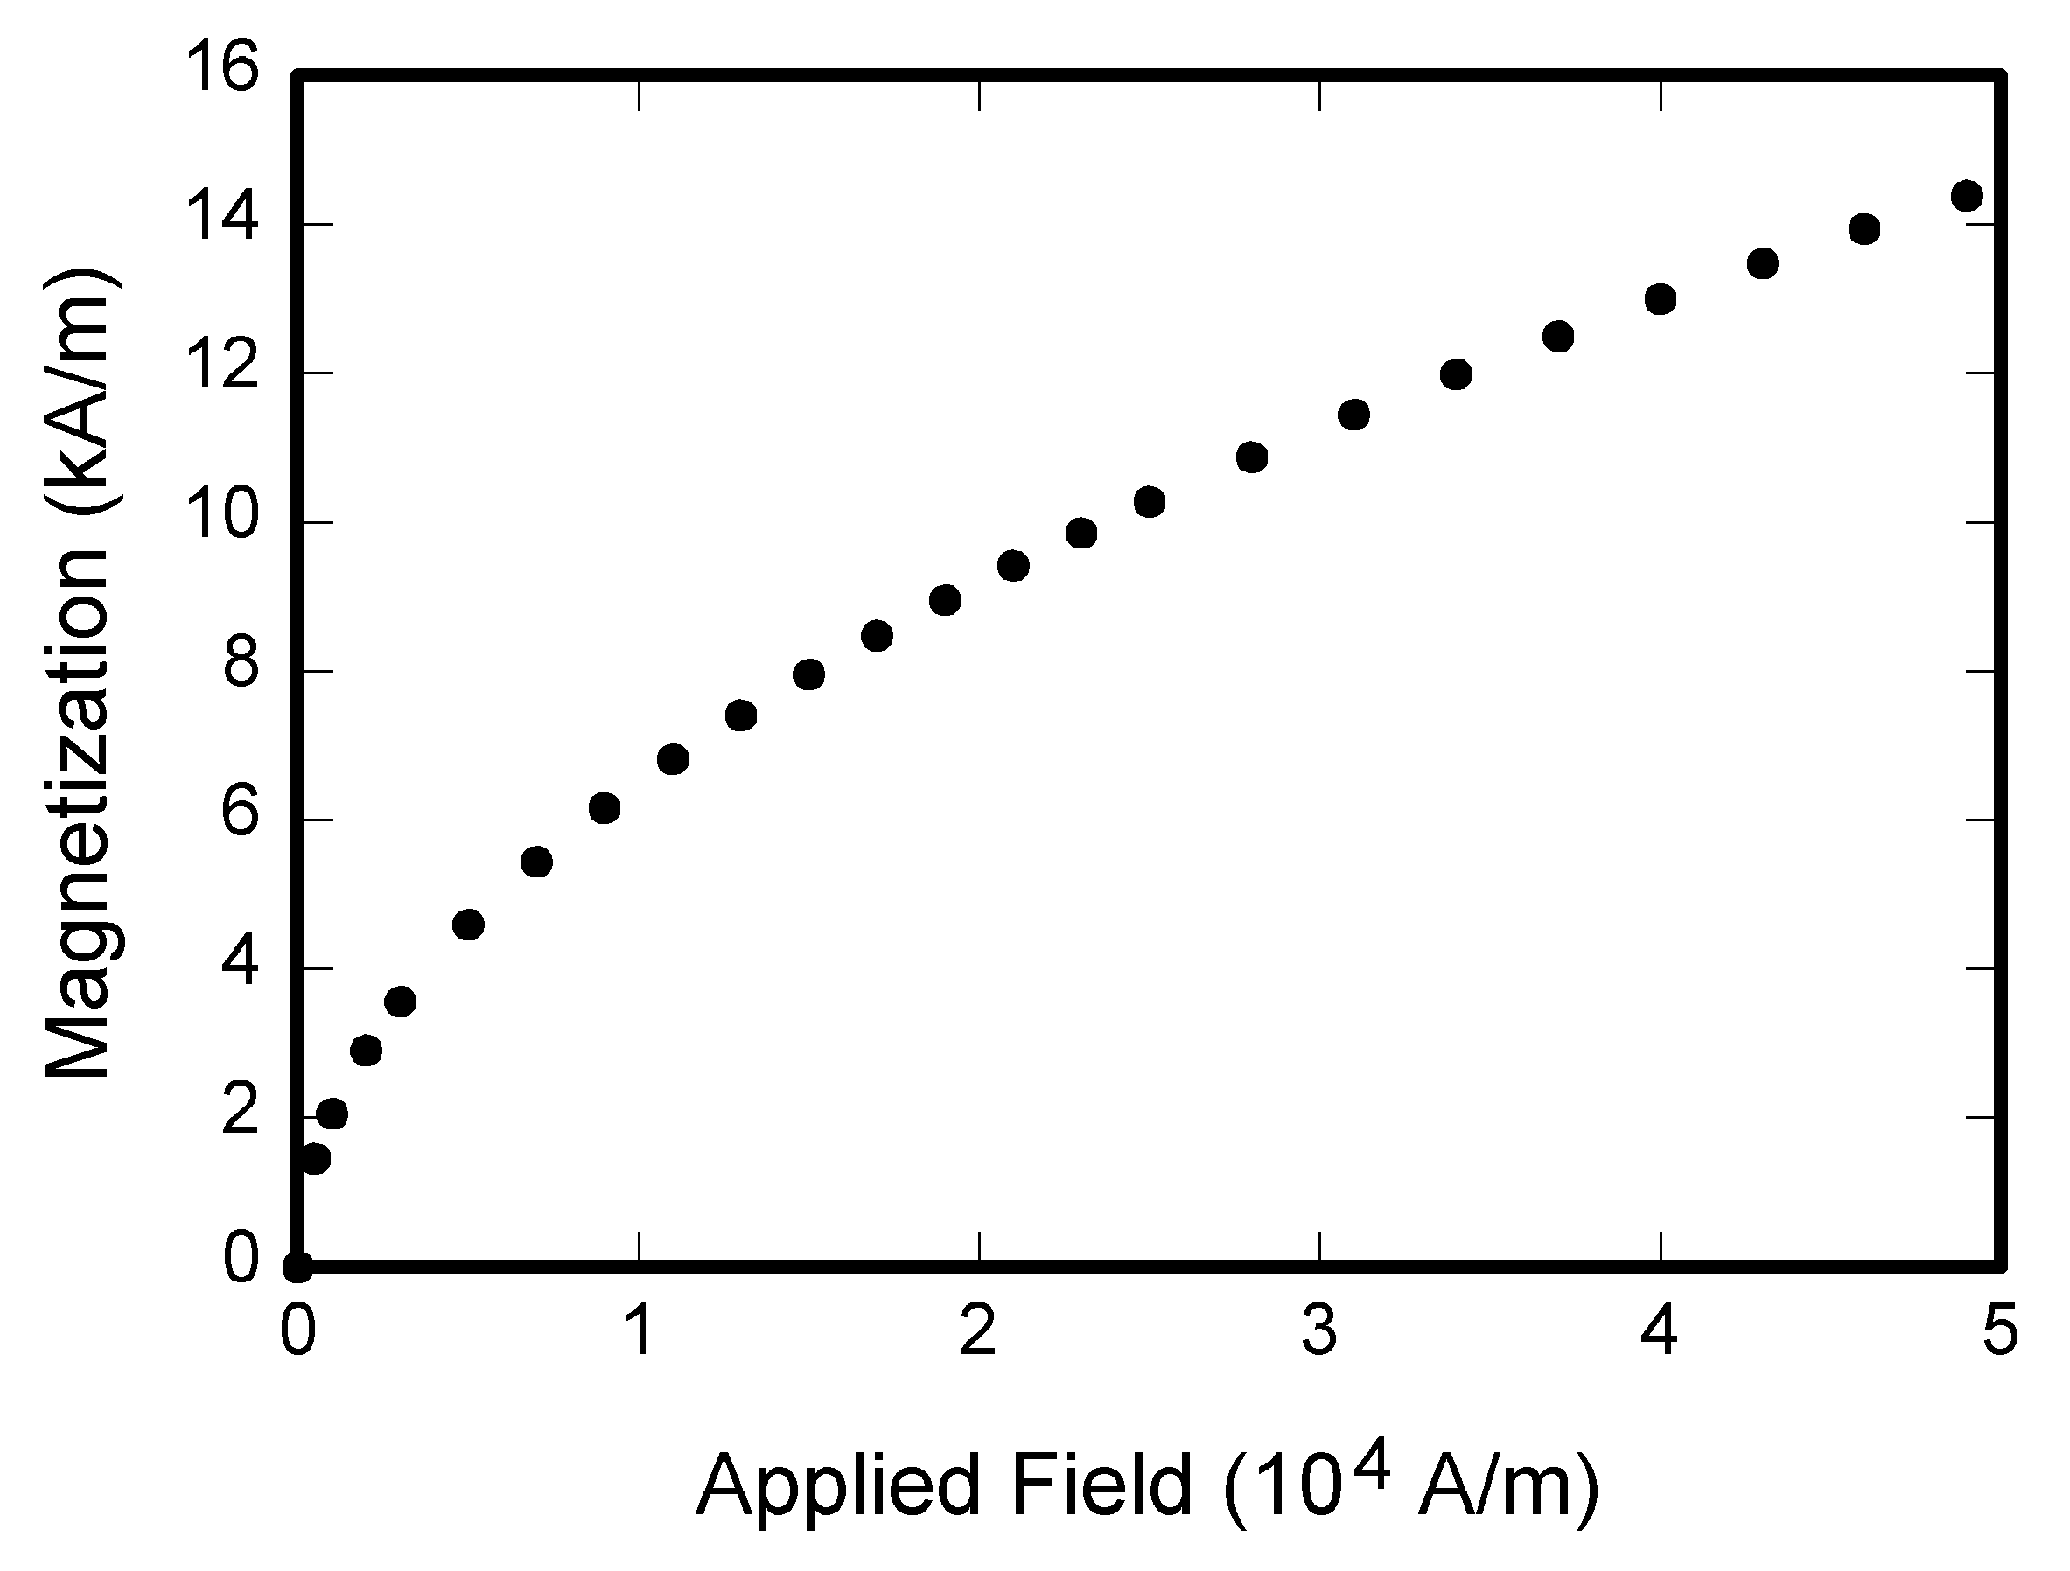
\includegraphics{fig1.png}}
% \caption{Example of a figure caption.}
% \label{fig}
% \end{figure}

% Figure Labels: Use 8 point Times New Roman for Figure labels. Use words 
% rather than symbols or abbreviations when writing Figure axis labels to 
% avoid confusing the reader. As an example, write the quantity 
% ``Magnetization'', or ``Magnetization, M'', not just ``M''. If including 
% units in the label, present them within parentheses. Do not label axes only 
% with units. In the example, write ``Magnetization (A/m)'' or ``Magnetization 
% \{A[m(1)]\}'', not just ``A/m''. Do not label axes with a ratio of 
% quantities and units. For example, write ``Temperature (K)'', not 
% ``Temperature/K''.

% \section*{Acknowledgment}

% The preferred spelling of the word ``acknowledgment'' in America is without 
% an ``e'' after the ``g''. Avoid the stilted expression ``one of us (R. B. 
% G.) thanks $\ldots$''. Instead, try ``R. B. G. thanks$\ldots$''. Put sponsor 
% acknowledgments in the unnumbered footnote on the first page.

% \section*{References}
% The \cite{jay1981gender}
% Please number citations consecutively within brackets \cite{b1}. The 
% sentence punctuation follows the bracket \cite{b2}. Refer simply to the reference 
% number, as in \cite{b3}---do not use ``Ref. \cite{b3}'' or ``reference \cite{b3}'' except at 
% the beginning of a sentence: ``Reference \cite{b3} was the first $\ldots$''

% Number footnotes separately in superscripts. Place the actual footnote at 
% the bottom of the column in which it was cited. Do not put footnotes in the 
% abstract or reference list. Use letters for table footnotes.

% Unless there are six authors or more give all authors' names; do not use 
% ``et al.''. Papers that have not been published, even if they have been 
% submitted for publication, should be cited as ``unpublished'' \cite{b4}. Papers 
% that have been accepted for publication should be cited as ``in press'' \cite{b5}. 
% Capitalize only the first word in a paper title, except for proper nouns and 
% element symbols.

% For papers published in translation journals, please give the English 
% citation first, followed by the original foreign-language citation \cite{b6}.

% \begin{thebibliography}{00}
% \bibitem{b1} G. Eason, B. Noble, and I. N. Sneddon, ``On certain integrals of Lipschitz-Hankel type involving products of Bessel functions,'' Phil. Trans. Roy. Soc. London, vol. A247, pp. 529--551, April 1955.
% \bibitem{b2} J. Clerk Maxwell, A Treatise on Electricity and Magnetism, 3rd ed., vol. 2. Oxford: Clarendon, 1892, pp.68--73.
% \bibitem{b3} I. S. Jacobs and C. P. Bean, ``Fine particles, thin films and exchange anisotropy,'' in Magnetism, vol. III, G. T. Rado and H. Suhl, Eds. New York: Academic, 1963, pp. 271--350.
% \bibitem{b4} K. Elissa, ``Title of paper if known,'' unpublished.
% \bibitem{b5} R. Nicole, ``Title of paper with only first word capitalized,'' J. Name Stand. Abbrev., in press.
% \bibitem{b6} Y. Yorozu, M. Hirano, K. Oka, and Y. Tagawa, ``Electron spectroscopy studies on magneto-optical media and plastic substrate interface,'' IEEE Transl. J. Magn. Japan, vol. 2, pp. 740--741, August 1987 [Digests 9th Annual Conf. Magnetics Japan, p. 301, 1982].
% \bibitem{b7} M. Young, The Technical Writer's Handbook. Mill Valley, CA: University Science, 1989.
% \bibitem{b8} D. P. Kingma and M. Welling, ``Auto-encoding variational Bayes,'' 2013, arXiv:1312.6114. [Online]. Available: https://arxiv.org/abs/1312.6114
% \bibitem{b9} S. Liu, ``Wi-Fi Energy Detection Testbed (12MTC),'' 2023, gitHub repository. [Online]. Available: https://github.com/liustone99/Wi-Fi-Energy-Detection-Testbed-12MTC
% \bibitem{b10} ``Treatment episode data set: discharges (TEDS-D): concatenated, 2006 to 2009.'' U.S. Department of Health and Human Services, Substance Abuse and Mental Health Services Administration, Office of Applied Studies, August, 2013, DOI:10.3886/ICPSR30122.v2
% \bibitem{b11} K. Eves and J. Valasek, ``Adaptive control for singularly perturbed systems examples,'' Code Ocean, Aug. 2023. [Online]. Available: https://codeocean.com/capsule/4989235/tree
% \end{thebibliography}

% \vspace{12pt}
% \color{red}
% IEEE conference templates contain guidance text for composing and formatting conference papers. Please ensure that all template text is removed from your conference paper prior to submission to the conference. Failure to remove the template text from your paper may result in your paper not being published.

